\documentclass[conference]{IEEEtran}

% --- Packages ---
\usepackage[T1]{fontenc}
\usepackage[utf8]{inputenc}
\usepackage{cite}
\usepackage{amsmath,amssymb,amsfonts}
\usepackage{graphicx}
\usepackage{booktabs}
\usepackage{array}
\usepackage{hyperref}
\usepackage{xcolor}

% Optional: for algorithms
% \usepackage{algorithm}
% \usepackage{algorithmic}

% Optional: for subfigures
% \usepackage{subcaption}

\begin{document}

\title{Object Classification with Small Data: A Case Study on Rat Images}

\author{
\IEEEauthorblockN{Nathaniel McComas}
\IEEEauthorblockA{
College of Natural and Health Sciences\\
University of Hawai`i at Hilo\\
Hilo, Hawai`i, USA\\
nmccomas@hawaii.edu
}
}

\maketitle

\begin{abstract}
    One of the central challenges in machine learning and other data science fields is obtaining enough labeled data to train a model effectively. This challenge is especially pronounced in specialized domains, where collecting and annotating data can be expensive and time consuming. This paper studies object classification with small-data constraints through a case study on classifying images of pet rats. We compare transfer-learned CNNs with different augmentation techniques, learning rates, and backbone-freezing schedules to identify which combinations produce the best generalization to unseen data. The resulting study concludes with practical guidance for small-data image classification problems in which dataset size and class imbalance present substantial obstacles.
\end{abstract}

\begin{IEEEkeywords}
small data, object classification, data augmentation, model architecture
\end{IEEEkeywords}

\section{Introduction}
Object classification remains one of the core tasks in computer vision, and deep convolutional models have achieved strong performance on large-scale benchmarks such as ImageNet \cite{deng2009imagenet, krizhevsky2012imagenet}. However, successful image classification systems are often built on datasets that are far larger and more diverse than what is available in many real-world settings. In specialized domains, obtaining enough labeled data to train a robust model can be difficult, expensive, or both. Small datasets also amplify practical problems such as overfitting, spurious correlations, and poor generalization to new environments or individuals \cite{goodfellow2016deep}.

This paper studies object classification with limited data through a case study on pet rat images. Rather than asking only which architecture is strongest in general, we examine which design choices produce the best generalization to unseen data. We focus on transfer learning \cite{pan2010transfer}, augmentation \cite{shorten2019augmentation}, model family and size \cite{he2016resnet, howard2017mobilenets, tan2019efficientnet}, and simple training-time choices such as learning rate and how long to keep the feature extractor/backbone frozen. The goal is not to identify a single best model and/or set of design choices, but rather to understand how these factors interact and which factor is most important for improving generalization in the small-data regime.

\subsection{Related Work}
There has been a significant amount of research on techniques for improving model performance with small datasets. Two of the most common approaches are transfer learning, in which a model pre-trained on a large dataset is fine-tuned on a smaller target dataset \cite{pan2010transfer}, and data augmentation, which creates additional training examples by applying label-preserving transformations such as cropping, flipping, rotating, and color jittering \cite{shorten2019augmentation}. Often, these techniques are combined so that a model starts from broadly useful visual features while also seeing more variation during training \cite{pan2010transfer, shorten2019augmentation}.

\subsection{Paper Organization}
The rest of this paper is organized as follows: In Section II, we provide further background on object classification with small datasets and briefly discuss our dataset. In Section III, we describe our methods, including the experimental setup and implementation details. In Section IV, we present the results of our experiments, including performance metrics and comparisons between different techniques. In Section V, we discuss the implications of our results, including the strengths and limitations of our approach. Finally, in Section VI, we summarize the main takeaways from our work and potential directions for future research.

\section{Background}
There are several challenges associated with object classification using small datasets. These include limited data availability, elevated risk of overfitting, and difficulty generalizing to unseen examples. In this section, we summarize the concepts most relevant to our study: transfer learning, data augmentation, and architecture selection.

\subsection{Techniques for Small Data}
When working with small datasets, some of the most common techniques for improving performance and generalization include transfer learning, data augmentation, and careful selection of model architecture and training parameters.

\subsubsection{Transfer Learning}
As mentioned in the introduction, transfer learning uses a model pre-trained on a large source dataset and adapts it to a smaller target dataset \cite{pan2010transfer}. This approach allows the model to reuse previously learned visual representations, which is especially helpful when the target dataset is too small to support strong representation learning from scratch. For example, models pre-trained on ImageNet learn generic features such as edges, textures, and part-level patterns that transfer well across many visual tasks \cite{deng2009imagenet}. By fine-tuning such models on our rat dataset, we are essentially leveraging the knowledge encoded in the pre-trained weights to jump-start learning and improve generalization, even with limited data.

Without transfer learning, training a deep network from scratch on a small dataset would be much more likely to lead to severe overfitting, since the model may have far more parameters than the data can constrain effectively \cite{goodfellow2016deep}. For that reason, pre-trained initialization is a natural default for this project.

\subsubsection{Data Augmentation}
Data augmentation is a technique used to artificially increase the effective size of a training dataset by applying label-preserving transformations to existing data. This can help improve model performance by providing more variation during training and reducing overfitting. In small datasets, a model may otherwise learn to associate specific poses, orientations, environments, or lighting conditions with the class labels, which can lead to poor generalization. Applying transformations such as random cropping, flipping, rotating, and color jittering can help the model learn more robust features that are less tied to those incidental conditions.

Beyond these basic transformations, more advanced augmentation strategies such as random erasing and composition-based methods (e.g., combining multiple images within a single training example) can further regularize training, although we will not fully explore these techniques in this work \cite{shorten2019augmentation}.

\begin{figure}
    \centering
    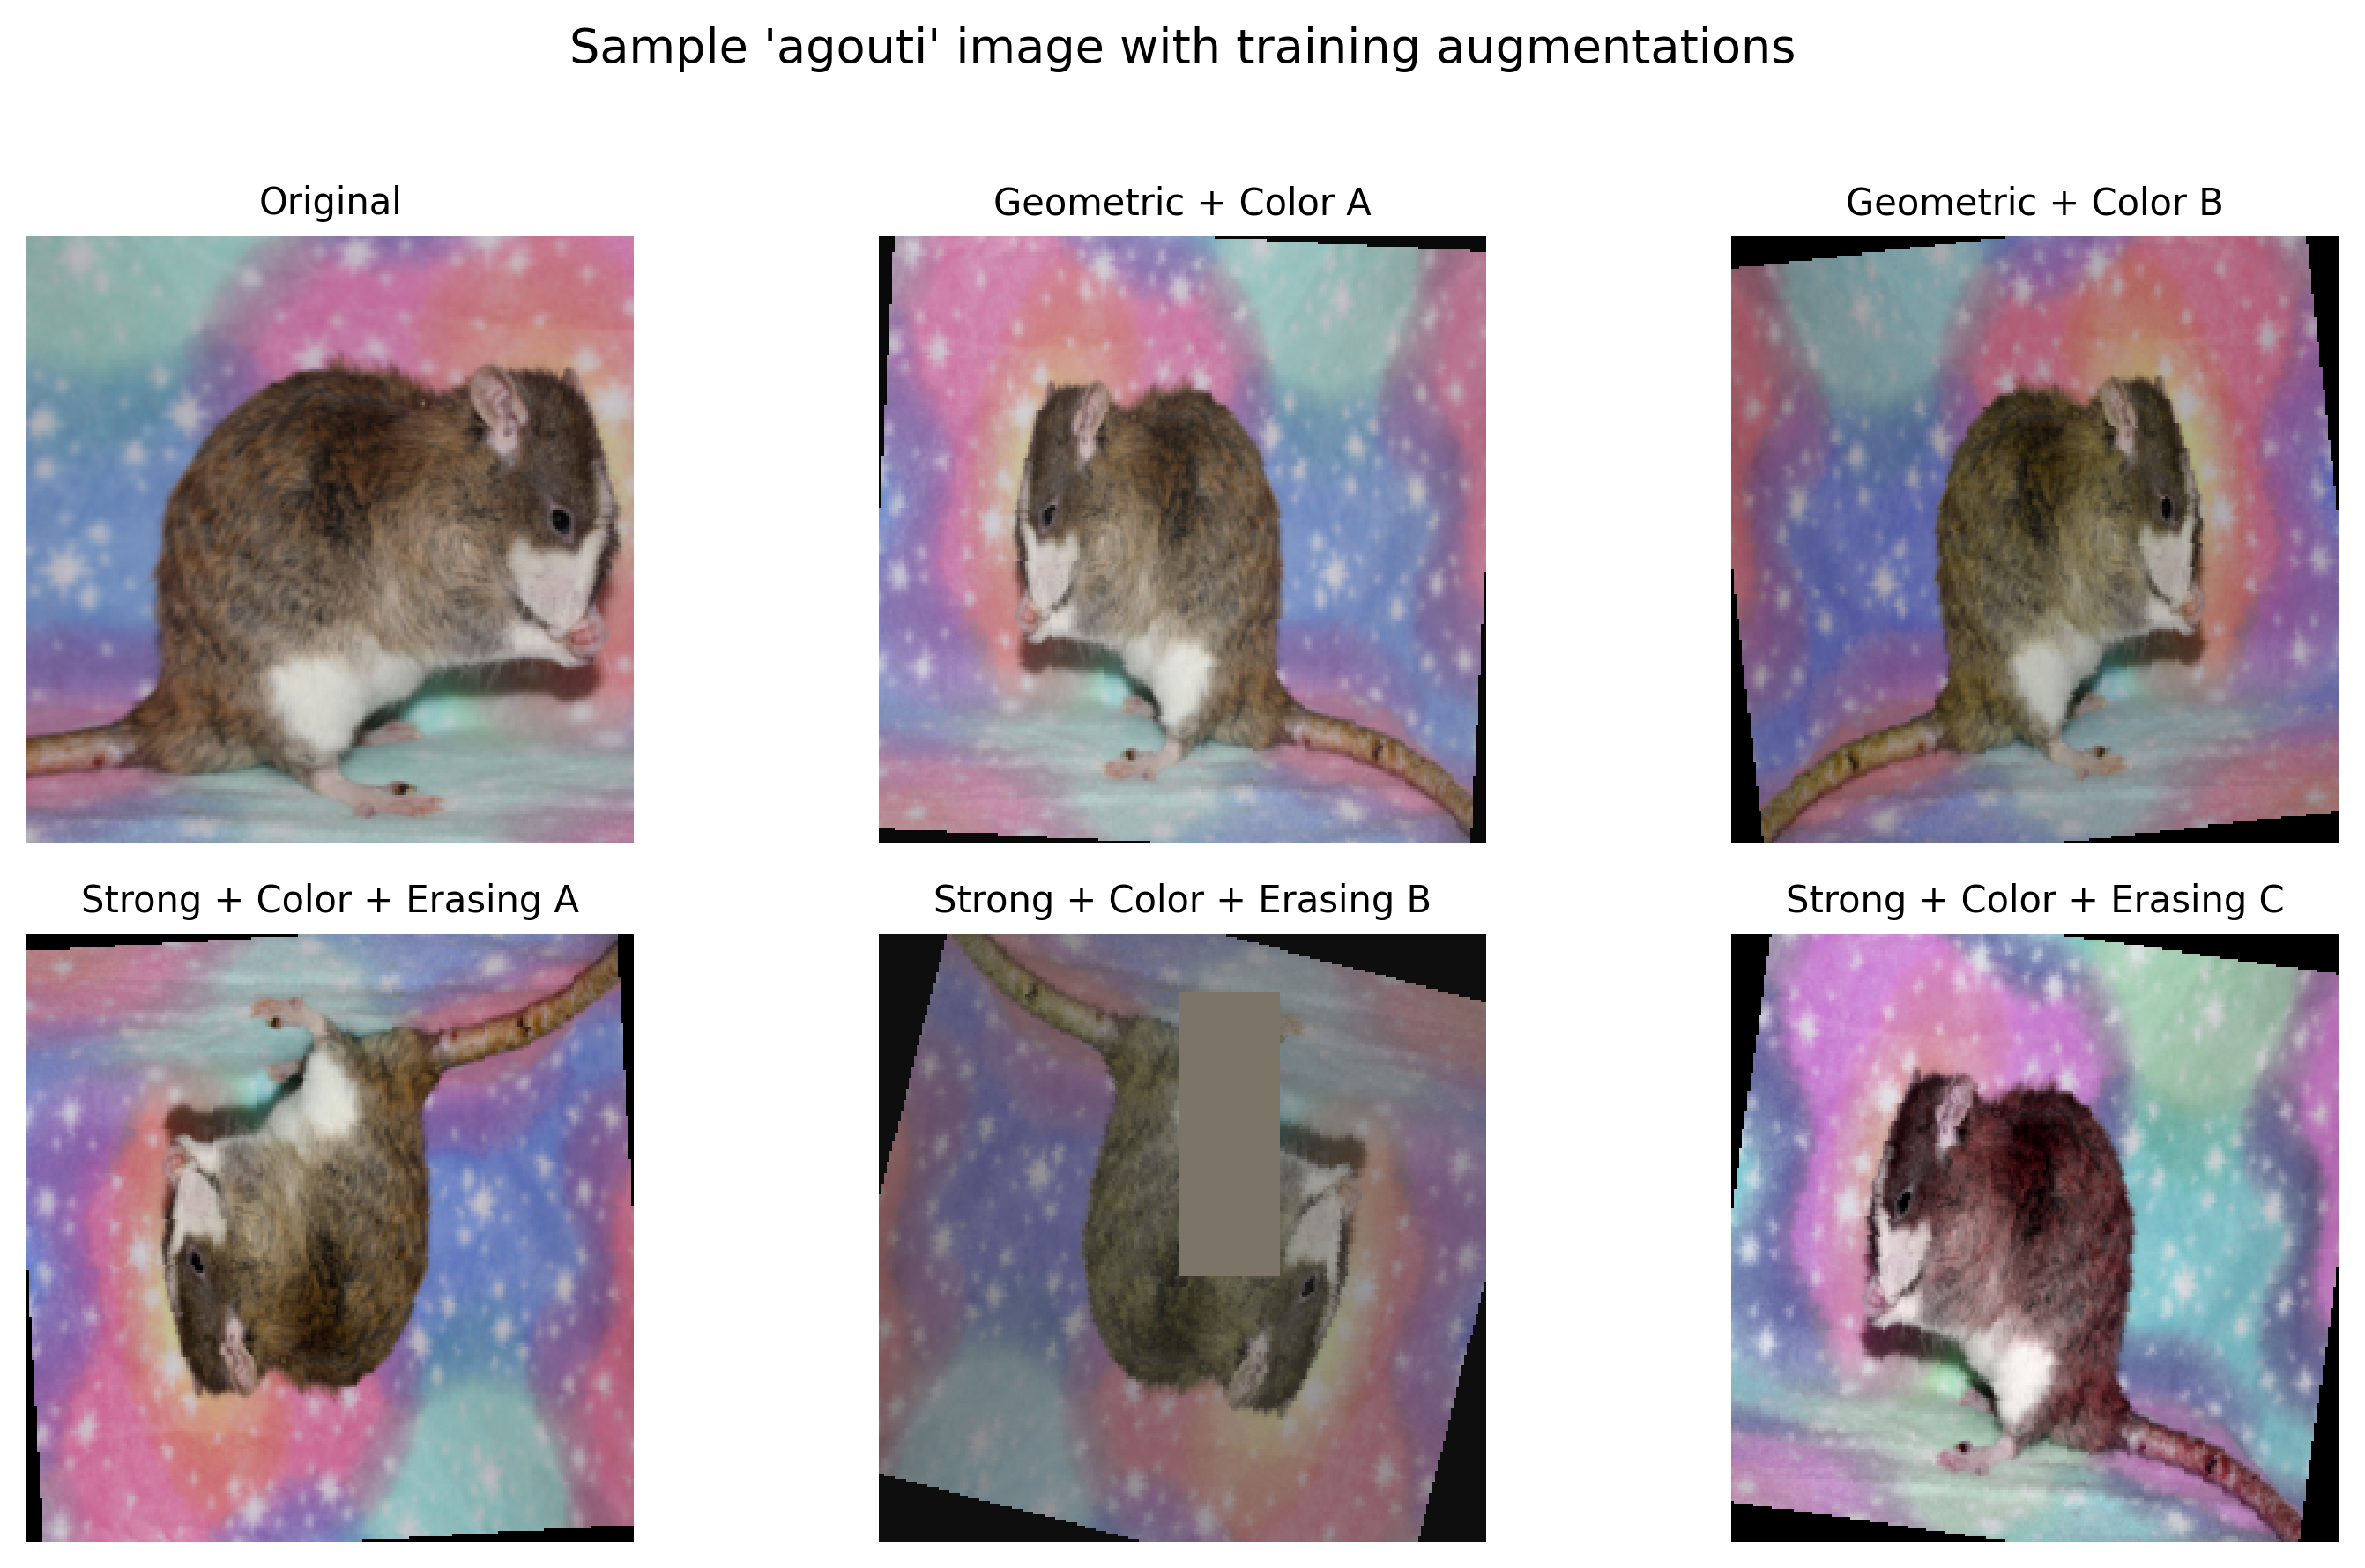
\includegraphics[width=0.8\linewidth]{example_augmented_images.png}
    \caption{Example of training-time augmentation applied to one rat image from our dataset. The top-left panel shows the original image after resizing and center cropping for display, while the remaining panels show representative outputs produced by two different augmentation pipelines. Thanks to Little Paws Rattery for allowing us to use this image.}
    \label{fig:augmentation_examples}
\end{figure}

\subsubsection{Model Architecture Considerations}
When working with small datasets, the choice of model architecture can have a significant impact on performance. Models with too many parameters may be prone to overfitting, while models that are too simple may lack the capacity to learn meaningful patterns from the data \cite{goodfellow2016deep}. Therefore, it is important to consider architectural complexity in relation to dataset size. In general, regularization methods such as dropout and/or weight decay can also help reduce overfitting when data are limited \cite{srivastava2014dropout}.

Besides model size, the specific architecture can also play a role. Convolutional neural networks (CNNs) are commonly used for image classification tasks due to their ability to learn spatial hierarchies of features \cite{lecun1998gradient, krizhevsky2012imagenet}. However, even within CNNs, there are many different architectures to choose from, such as ResNet \cite{he2016resnet}, EfficientNet \cite{tan2019efficientnet}, and MobileNet \cite{howard2017mobilenets}, each with its own trade-offs in terms of complexity and performance. When working with small datasets, it may be beneficial to carefully select an architecture that is well-suited to the task and the amount of data available.

\subsection{Dataset}

Our dataset consists of images of pet rats collected from breeder websites and public social-media pages, with permission granted for their use in this project. Specific breeder credits are provided in the Acknowledgment section. The dataset contains images from five coat-based classes:

\begin{enumerate}
    \item Agouti
    \item Black
    \item Blue
    \item Marten
    \item Double Rex/Hairless
\end{enumerate}

In total, the dataset contains 554 images organized under 129 immediate nested folders. Most of these folders correspond to individual rats, while a small number are class-level assortment folders used for sparse examples. The class image counts are 136 Agouti, 122 Black, 113 Blue, 138 Marten, and 45 Double Rex/Hairless. Counting the immediate nested folders used by the split procedure yields 34 Agouti folders, 17 Black, 26 Blue, 35 Marten, and 17 Double Rex/Hairless.

There are a number of important considerations regarding this dataset that could impact model performance and generalization.

\subsubsection{Individuals and Environments}

Most folders in the dataset correspond to a single identified rat, which lets us reason about generalization across individuals rather than only across images. In addition, each class contains an assortment folder that groups together rats from that class when only one or two images are available for a given individual instead of creating many separate sparse folders. This preserves scarce data, but it also makes per-individual accounting less precise for that subset of the dataset.

Among the five classes, there is an imbalance in the number of individuals represented, with some classes containing many more individuals than others. Furthermore, some classes simply have much fewer images overall, which could make it difficult for models to learn robust features for those classes. This imbalance could lead to models learning spurious correlations that are specific to the individuals or environments represented in the dataset, rather than learning generalizable features that are relevant to the class as a whole.

It is our hope that strong data augmentation and careful model architecture choices can help mitigate these issues and allow the models to learn more robust features that generalize well to new individuals and environments. However, these are important limitations to keep in mind when interpreting the results of our experiments.

\subsubsection{Juveniles}

A very large portion of the rats are juveniles, since many of the pictures shared by participating breeders are of new litters. This could lead to models learning to identify juvenile features rather than features specific to the intended class, which could also limit generalization to new images of adult rats within the same class.

Again, we hope that strong data augmentation and careful model architecture choices can help mitigate this issue and allow the models to learn more robust features that generalize well to both juvenile and adult rats. However, this is another important limitation to keep in mind when interpreting the results of our experiments.

\subsubsection{Note about Rat Genetics and Classification}

It is important to note that the classification of rats into these 5 different classes is not a strictly scientific classification based on genetics, but rather a more informal classification based on physical appearance and traits. It is also important to note that many of these classes are not mutually exclusive, and there may be some overlap between them. For example, a rat could simultaneously be a blue, marten, and agouti. This is because these classes are based on physical traits that can be influenced by multiple genetic factors, and there is not always a clear-cut distinction between them. Therefore, it is important to keep in mind that the classification of rats into these classes is somewhat subjective and may not always be consistent across different individuals or breeders.

In order to determine the class labels for our dataset, we chose our own hierarchy of traits to use for classification, which is based on the visible characteristics of the rats in the images. We acknowledge that this classification is not perfect and may not be universally accepted, but it provides a consistent framework for labeling our dataset and conducting our experiments. In order, we used the following hierarchy of traits for classification:

\begin{enumerate}
    \item Double Rex/Hairless: If the rat has a double rex coat OR it is hairless, it is classified as a Double Rex/Hairless. Although these are not necessarily the same trait, they are grouped together for classification purposes. They are both characterized by partial or complete absence of fur. This trait is relatively easy to identify and classify based on visual characteristics, making it a clear choice for the first level of our classification hierarchy.
    \item Marten: If the rat has a marten coat, it is classified as a Marten. This is characterized by dark coloration on the extremities (face, feet, tail) which fades into a lighter color on the body. This trait is relatively easy to identify and classify based on visual characteristics, making it a clear choice for the second level of our classification hierarchy. It is noteworthy that Martens more often have red eyes than other classes, which could be a confounding factor for classification.
    \item Blue: If the rat has a blue coat, it is classified as a Blue. Despite their name, they are often characterized by a partial or complete dark-gray coat, rarely with a bluish tint. This trait is relatively easy to identify and classify based on visual characteristics, making it a clear choice for the third level of our classification hierarchy. However, it is noteworthy that Blues can overlap with Agoutis, in which case the Blue trait takes precedence in our hierarchy.
    \item Agouti: If the rat has an agouti coat and no other higher precedence traits (as defined above), it is classified as an Agouti. This is characterized by multiple hair bands of different colors on each individual hair, which creates a "wild-type" coat color that is often brown or gray with a speckled appearance. This trait, although visually distinct, can be more difficult to identify and classify than the other traits due to its variability and potential overlap with other classes (e.g., a rat could be both an Agouti and a Blue). Therefore, it is placed lower in the classification hierarchy than the more visually distinct traits.
    \item Black: If the rat has a black coat and no other higher precedence traits (as defined above), it is classified as a Black. This is characterized by a solid black coat color on parts of or the entire body. This trait is relatively easy to identify, however it is placed last in the classification hierarchy because it is the least visually informative trait. For example, a rat could be both a Black and a Marten, but the Marten trait would take precedence in our hierarchy because it provides more specific information about the coat pattern and coloration than the Black trait alone.
\end{enumerate}

\subsubsection{Dataset Splitting}

For our experiments, we split the dataset into training, validation, and test sets. The training set is used for parameter updates. The validation set is used for early stopping and for comparing configurations during the sweep. The test set remains disjoint from training and validation and is evaluated only after a run has finished training, so it does not influence gradient updates or checkpoint selection.

The split is identity-based rather than image-based: each rat folder is assigned wholly to one split. This design is intended to test whether a model can generalize to unseen rats rather than merely unseen photographs of previously seen rats. The target split ratios are 60\% training, 15\% validation, and 25\% test.

Because the split operates on identity folders and uses best-effort allocation for small classes, the realized split is not exactly proportional at the image level. In our dataset, the resulting split contains 311 training images, 81 validation images, and 162 test images, corresponding to 77, 20, and 32 immediate nested folders respectively.

\section{Methods}

To investigate object classification with small datasets, we designed a controlled experiment around our dataset and varied only a small set of training factors at a time. All candidate models used ImageNet-pretrained weights \cite{deng2009imagenet}, and each run replaced the final classification head to predict the five dataset classes. We then compared families, model sizes, learning rates, augmentation pipelines, and backbone-freezing schedules while keeping the rest of the training recipe constant.

\subsection{Experimental Setup}

Our sweep evaluates four convolutional-network families: ResNet, MobileNet, EfficientNet, and DenseNet \cite{he2016resnet, howard2017mobilenets, tan2019efficientnet}. For each family, we test a smaller and a medium-sized variant, giving eight architectures in total. Each architecture is trained with two learning rates ($10^{-4}$ and $3 \times 10^{-3}$), two freezing schedules for the pre-trained backbone (freeze for the first 5 epochs or the first 15 epochs), and six augmentation pipelines ranging from minimal resizing and center cropping to strong geometric and color augmentation with random erasing \cite{shorten2019augmentation}. This yields 192 experiment configurations overall.

Across all runs, the batch size is fixed at 16. Training uses AdamW with weight decay of $10^{-4}$, a cosine-annealing learning-rate schedule, a maximum of 40 epochs, and early stopping after 10 epochs without improvement in validation loss. During the frozen-backbone phase, only the classifier head is updated; once the freeze period ends, the full network is fine-tuned. For each run, the best checkpoint is selected according to validation loss, and that trained model is then evaluated on both the validation and test splits.



\subsection{Implementation Details}

The project is implemented in PyTorch and Torchvision. Dataset loading is handled with \texttt{ImageFolder}, which assigns labels from the top-level class directories and recursively discovers images inside the nested identity folders. Identity-aware splitting is implemented before training so that all images from a given rat remain in the same subset.

Evaluation reports overall accuracy, macro-averaged precision, macro-averaged recall, and per-class counts of correct predictions, total examples, and predicted examples. These metrics are saved alongside the trained model weights for each run. Because the dataset is both small and somewhat imbalanced, we record macro-averaged metrics in addition to accuracy so that performance on minority classes is not obscured by stronger performance on the more represented classes.

\subsubsection{Data Augmentation Pipelines}

The six augmentation pipelines are as follows:

\begin{itemize}
    \item Minimal: Resize to 224x224 and normalize with ImageNet mean and std.
    \item Basic Geometric: Minimal + random horizontal flip and random rotation of up to 10 degrees.
    \item Strong Geometric: Minimal + random horizontal/vertical flips, and random rotation of up to 25 degrees.
    \item Basic Geometric + Color: Basic Geometric + random color jittering (brightness, contrast, saturation up to 0.15, hue up to 0.05)
    \item Strong Geometric + Color: Strong Geometric + random color jittering (brightness, contrast, saturation up to 0.3, hue up to 0.1)
    \item Strong Geometric + Color + Random Erasing: Strong Geometric + Color + random erasing with probability 0.25, scale (0.02, 0.15), and ratio (0.3, 3.3)
\end{itemize}

These are all implemented using the \texttt{torchvision.transforms} module, and the parameters were chosen to provide a range of augmentation strengths while still producing visually plausible images. See Figure \ref{fig:augmentation_examples} for examples of the outputs produced by these pipelines.

\subsubsection{Model Architectures with Size Variants}

As mentioned, we evaluate four CNN families with two size variants each. However, "small" and "medium" are relative terms that depend on the specific architecture. Hence, we define the size variants for each family as follows:

\begin{itemize}
    \item ResNet: ResNet-18 (small) and ResNet-34 (medium)
    \item MobileNet: MobileNetV3-Small (small) and MobileNetV2 (medium)
    \item EfficientNet: EfficientNet-B0 (small) and EfficientNet-B2 (medium)
    \item DenseNet: DenseNet-121 (small) and DenseNet-169 (medium)
\end{itemize}

For future reference, by "model architecture" or "architecture" we may be referring to the family (e.g., ResNet) or the specific size variant (e.g., ResNet-18).

\subsubsection{Splitting Details}

The split procedure begins by parsing each image path relative to the dataset root and extracting its class folder and immediate identity folder. It then builds a mapping from class name to rat name to the list of sample indices belonging to that rat. In other words, the split logic never operates on individual images directly; it operates on whole identity folders and then expands those folder assignments back into image indices.

For the experiments in this paper, the requested split ratios are 0.60, 0.15, and 0.25 for training, validation, and test respectively, with a fixed seed of 42. The procedure first normalizes the requested ratios so they sum to 1, then processes each class independently. Within each class, rat-folder names are sorted and then deterministically shuffled using a class-specific pseudorandom stream derived from the seed and class name. This means the split is reproducible across runs while still avoiding a bias from alphabetical folder order.

After shuffling, the procedure allocates how many identities from that class should go to each subset using a best-effort routine designed for small classes. If a class has only one identity folder, that identity is placed in training. If it has two identity folders, one is placed in training and one in test. If it has three or more identity folders, the allocator guarantees at least one training identity, one validation identity, and one test identity. Any remaining identities are distributed according to the requested ratios by combining floor-based allocation with a remainder rule that prioritizes larger unmet fractional targets. Once the rat folders assigned to each subset are known, all image indices from those folders are appended to the corresponding train, validation, or test index list.

The procedure also includes sanity checks. It raises an error if no training images can be created, and it raises errors when a nonzero validation or test ratio is requested but the dataset structure makes that impossible. Because the split is computed at the rat-folder level rather than the image level, all photographs of a given individual remain confined to a single subset, which is the key mechanism used to reduce leakage from near-duplicate images of the same rat across training, validation, and test data.

\section{Results}
This section will report the results of the full experiment sweep. In particular, we will compare model families, model sizes, augmentation strengths, and freezing schedules using validation and test accuracy, macro precision, and macro recall. We will also detail per-class performance and discuss how performance varies across classes with different levels of representation in the dataset. Finally, we will analyze which design choices appear most beneficial for improving generalization to unseen data and which choices seem to encourage overfitting or unstable generalization.

\subsection{Per Class Performance}
\label{sec:per_class_performance}

Likely the most interesting aspect of the results is how performance varies across classes within the dataset. Because the dataset is small and imbalanced with respect to the number of individuals and images per class, it is important to understand how well the models are able to learn robust features for each class and whether some classes are more difficult than others. This can provide insights into the strengths and weaknesses of the models and the dataset itself, as well as inform future efforts to improve performance on underrepresented classes. Refer to figure \ref{fig:per_class_pr} for a summary of per-class precision and recall averaged across all models and training configurations.

\begin{figure}
    \centering
    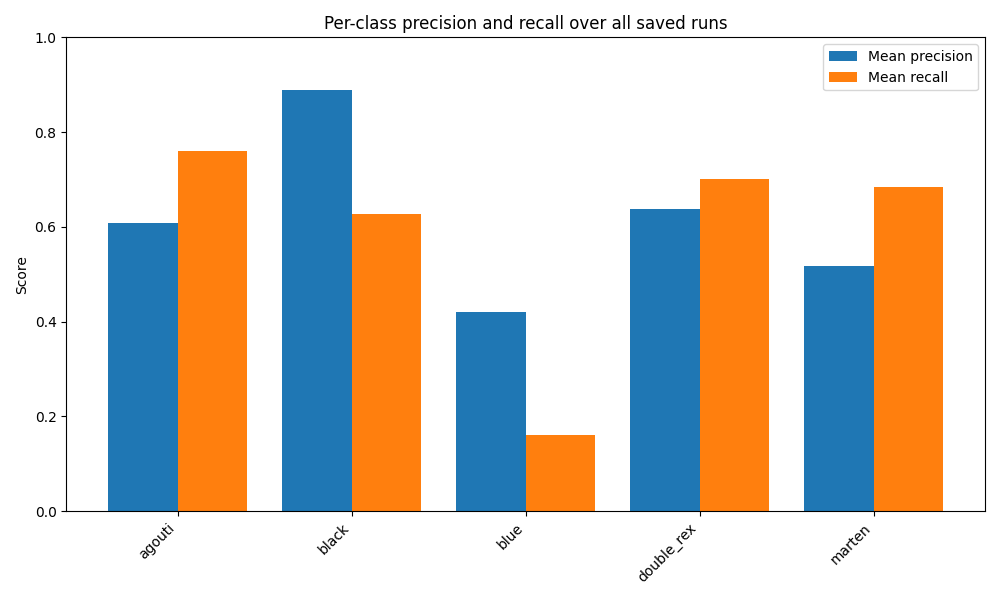
\includegraphics[width=\linewidth]{per_class_pr.png}
    \caption{Per-class precision and recall on the test set averaged across all models and training configurations. The Blue class shows the weakest precision and recall. The Agouti class shows the highest recall, and the Black class the highest precision. Despite the severe underrepresentation of the Double Rex/Hairless class, it has acceptable precision and recall, likely due to its distinctive visual features.}
    \label{fig:per_class_pr}
\end{figure}

The most notable trend is that the Blue class consistently shows the weakest performance across all models and training configurations. This suggests that the visual features of the Blue class may be more difficult for the models to capture and generalize from, which could be due to a number of factors such as variability in the appearance of Blue rats, overlap with other classes, or simply a lack of sufficient training examples for that class. Indeed, the Blue class is often confused with the Marten class, and the overall performance is poor enough that it appears likely that the overall performance of models is closely tied to their ability to learn features that separate Blue from Marten. See figure \ref{fig:blue_confusion} for the per-class misclassification of the Blue class across the 8 different model architectures. MobileNet v3 small only correctly classified 9.3\% of the Blue test images, making it the weakest architecture for that class. In comparison, EfficientNet B2 correctly classified 30.9\% of the Blue test images, making it the strongest architecture for that class.

\begin{figure}
    \centering
    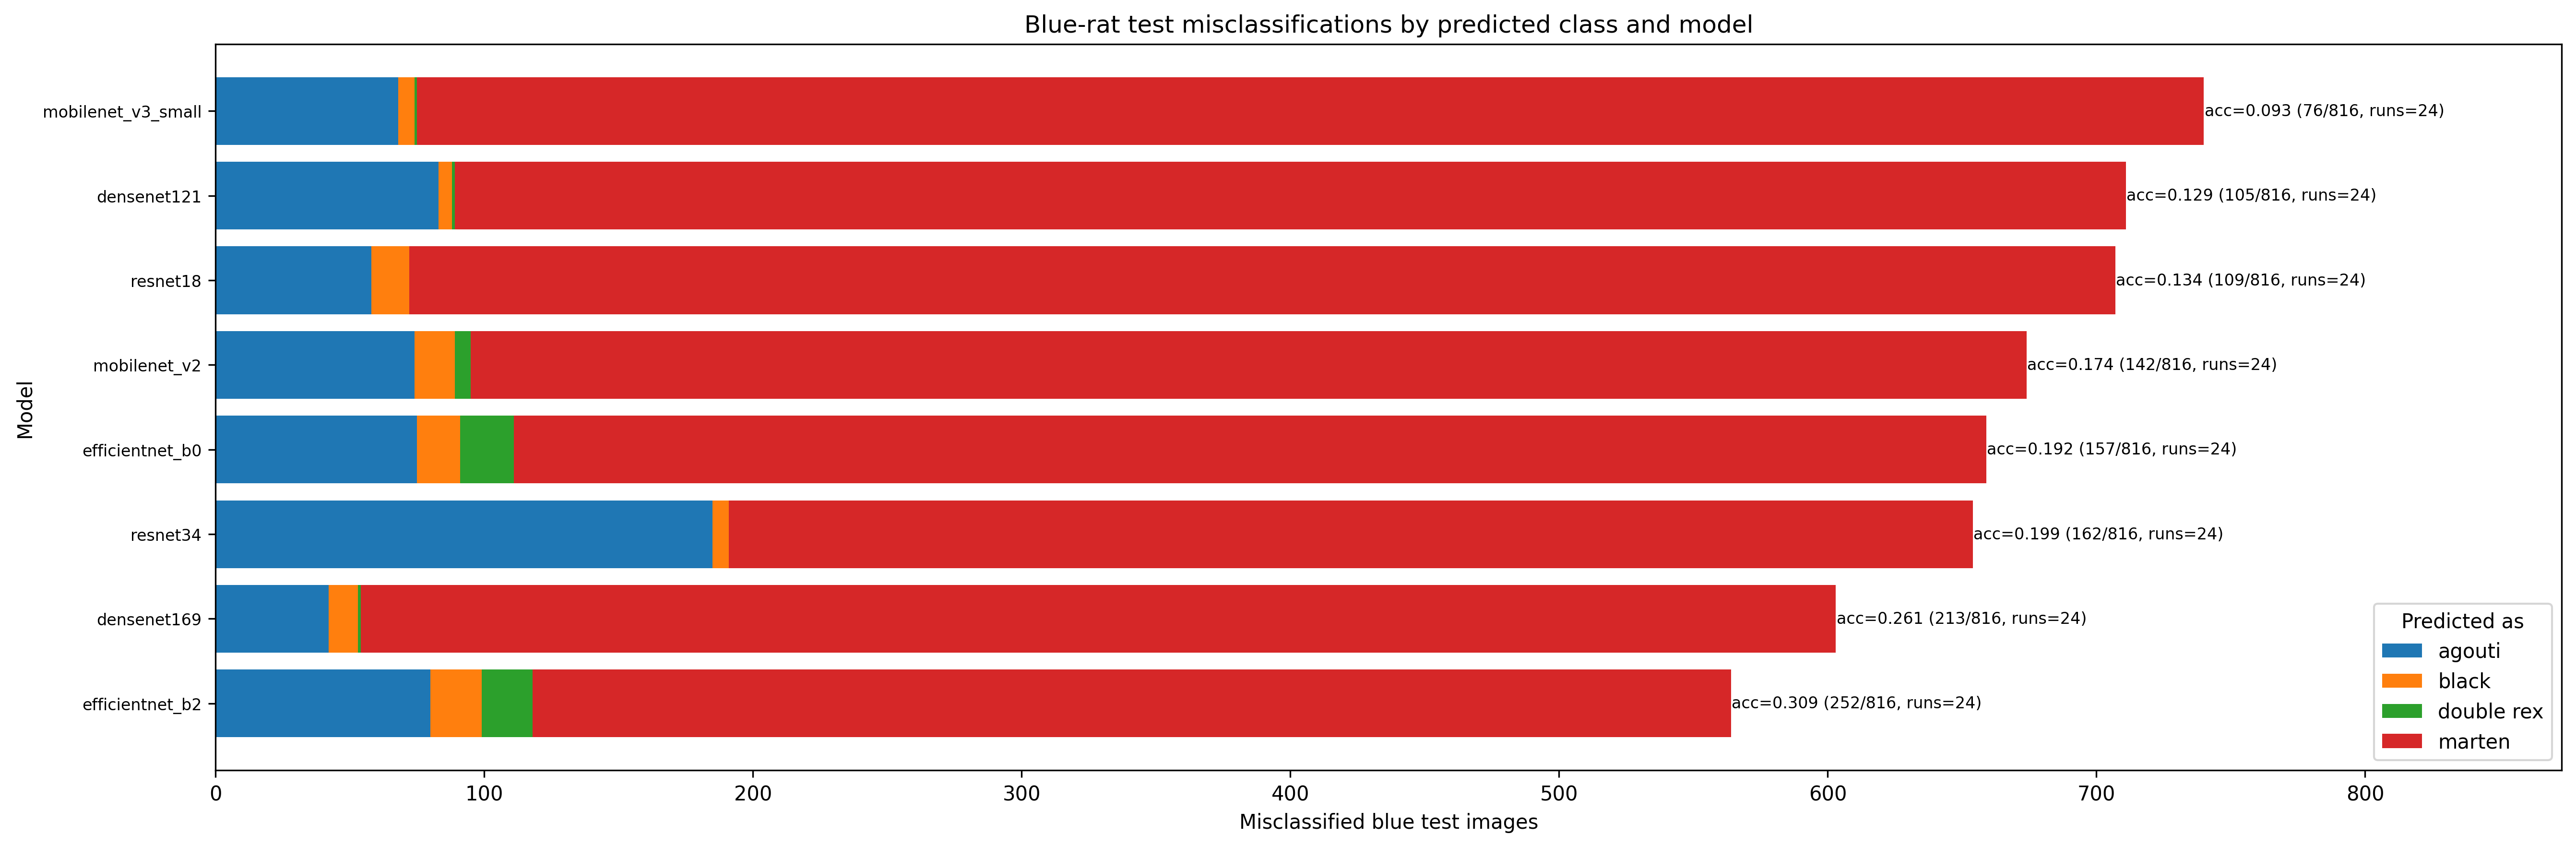
\includegraphics[width=\linewidth]{blue_confusion.png}
    \caption{Per-class misclassification for the Blue class across the 8 different model architectures. All of the Blue test images were run through the trained models, and the predicted classes were recorded and aggregated across each architecture. MobileNet v3 small only correctly classified 9.3\% of the Blue test images, making it the weakest architecture for that class. In comparison, EfficientNet B2 correctly classified 30.9\% of the Blue test images, making it the strongest architecture for that class.}
    \label{fig:blue_confusion}
\end{figure}

In contrast, the Agouti class shows the highest recall across all models and training configurations, which suggests that the models are able to learn robust features for that class and generalize well to unseen examples. The Black class shows the highest precision across all models and training configurations, which suggests that when the models do predict the Black class, they are often correct. However, the recall for the Black class is not as high as for the Agouti class, which suggests that the models may be missing some examples of the Black class or confusing them with other classes. Taken together, these results suggest that there are inherent differences in how easily the visual features of each class can be captured and generalized by the models, and that some classes may require more careful attention to improve performance than others.

\subsection{Model Family and Size Comparisons}

When comparing model families and sizes, we will analyze how different architectures perform in general and whether smaller or larger models tend to perform better in the small-data regime. We will also look at how the choice of architecture interacts with other design choices such as augmentation strength and freezing schedule. For example, it is possible that smaller models may benefit more from stronger augmentation or longer freezing schedules than larger models, which could help mitigate overfitting and improve generalization.

It first helps to directly compare the overall performance of the different model families and sizes. See figure \ref{fig:model_family_size_comparison} for a summary of test accuracy, macro precision, and macro recall averaged across all training configurations for each model architecture. Overall, EfficientNet B2 shows the strongest performance in general, while MobileNet v3 small shows the weakest performance. However, there is a small amount of variability within each model. This suggests that while architecture choice is important, it is not the only factor that influences performance in the small-data regime, and that other design choices such as augmentation strength and freezing schedule can also play a role in improving generalization to unseen data.

\begin{figure}
    \centering
    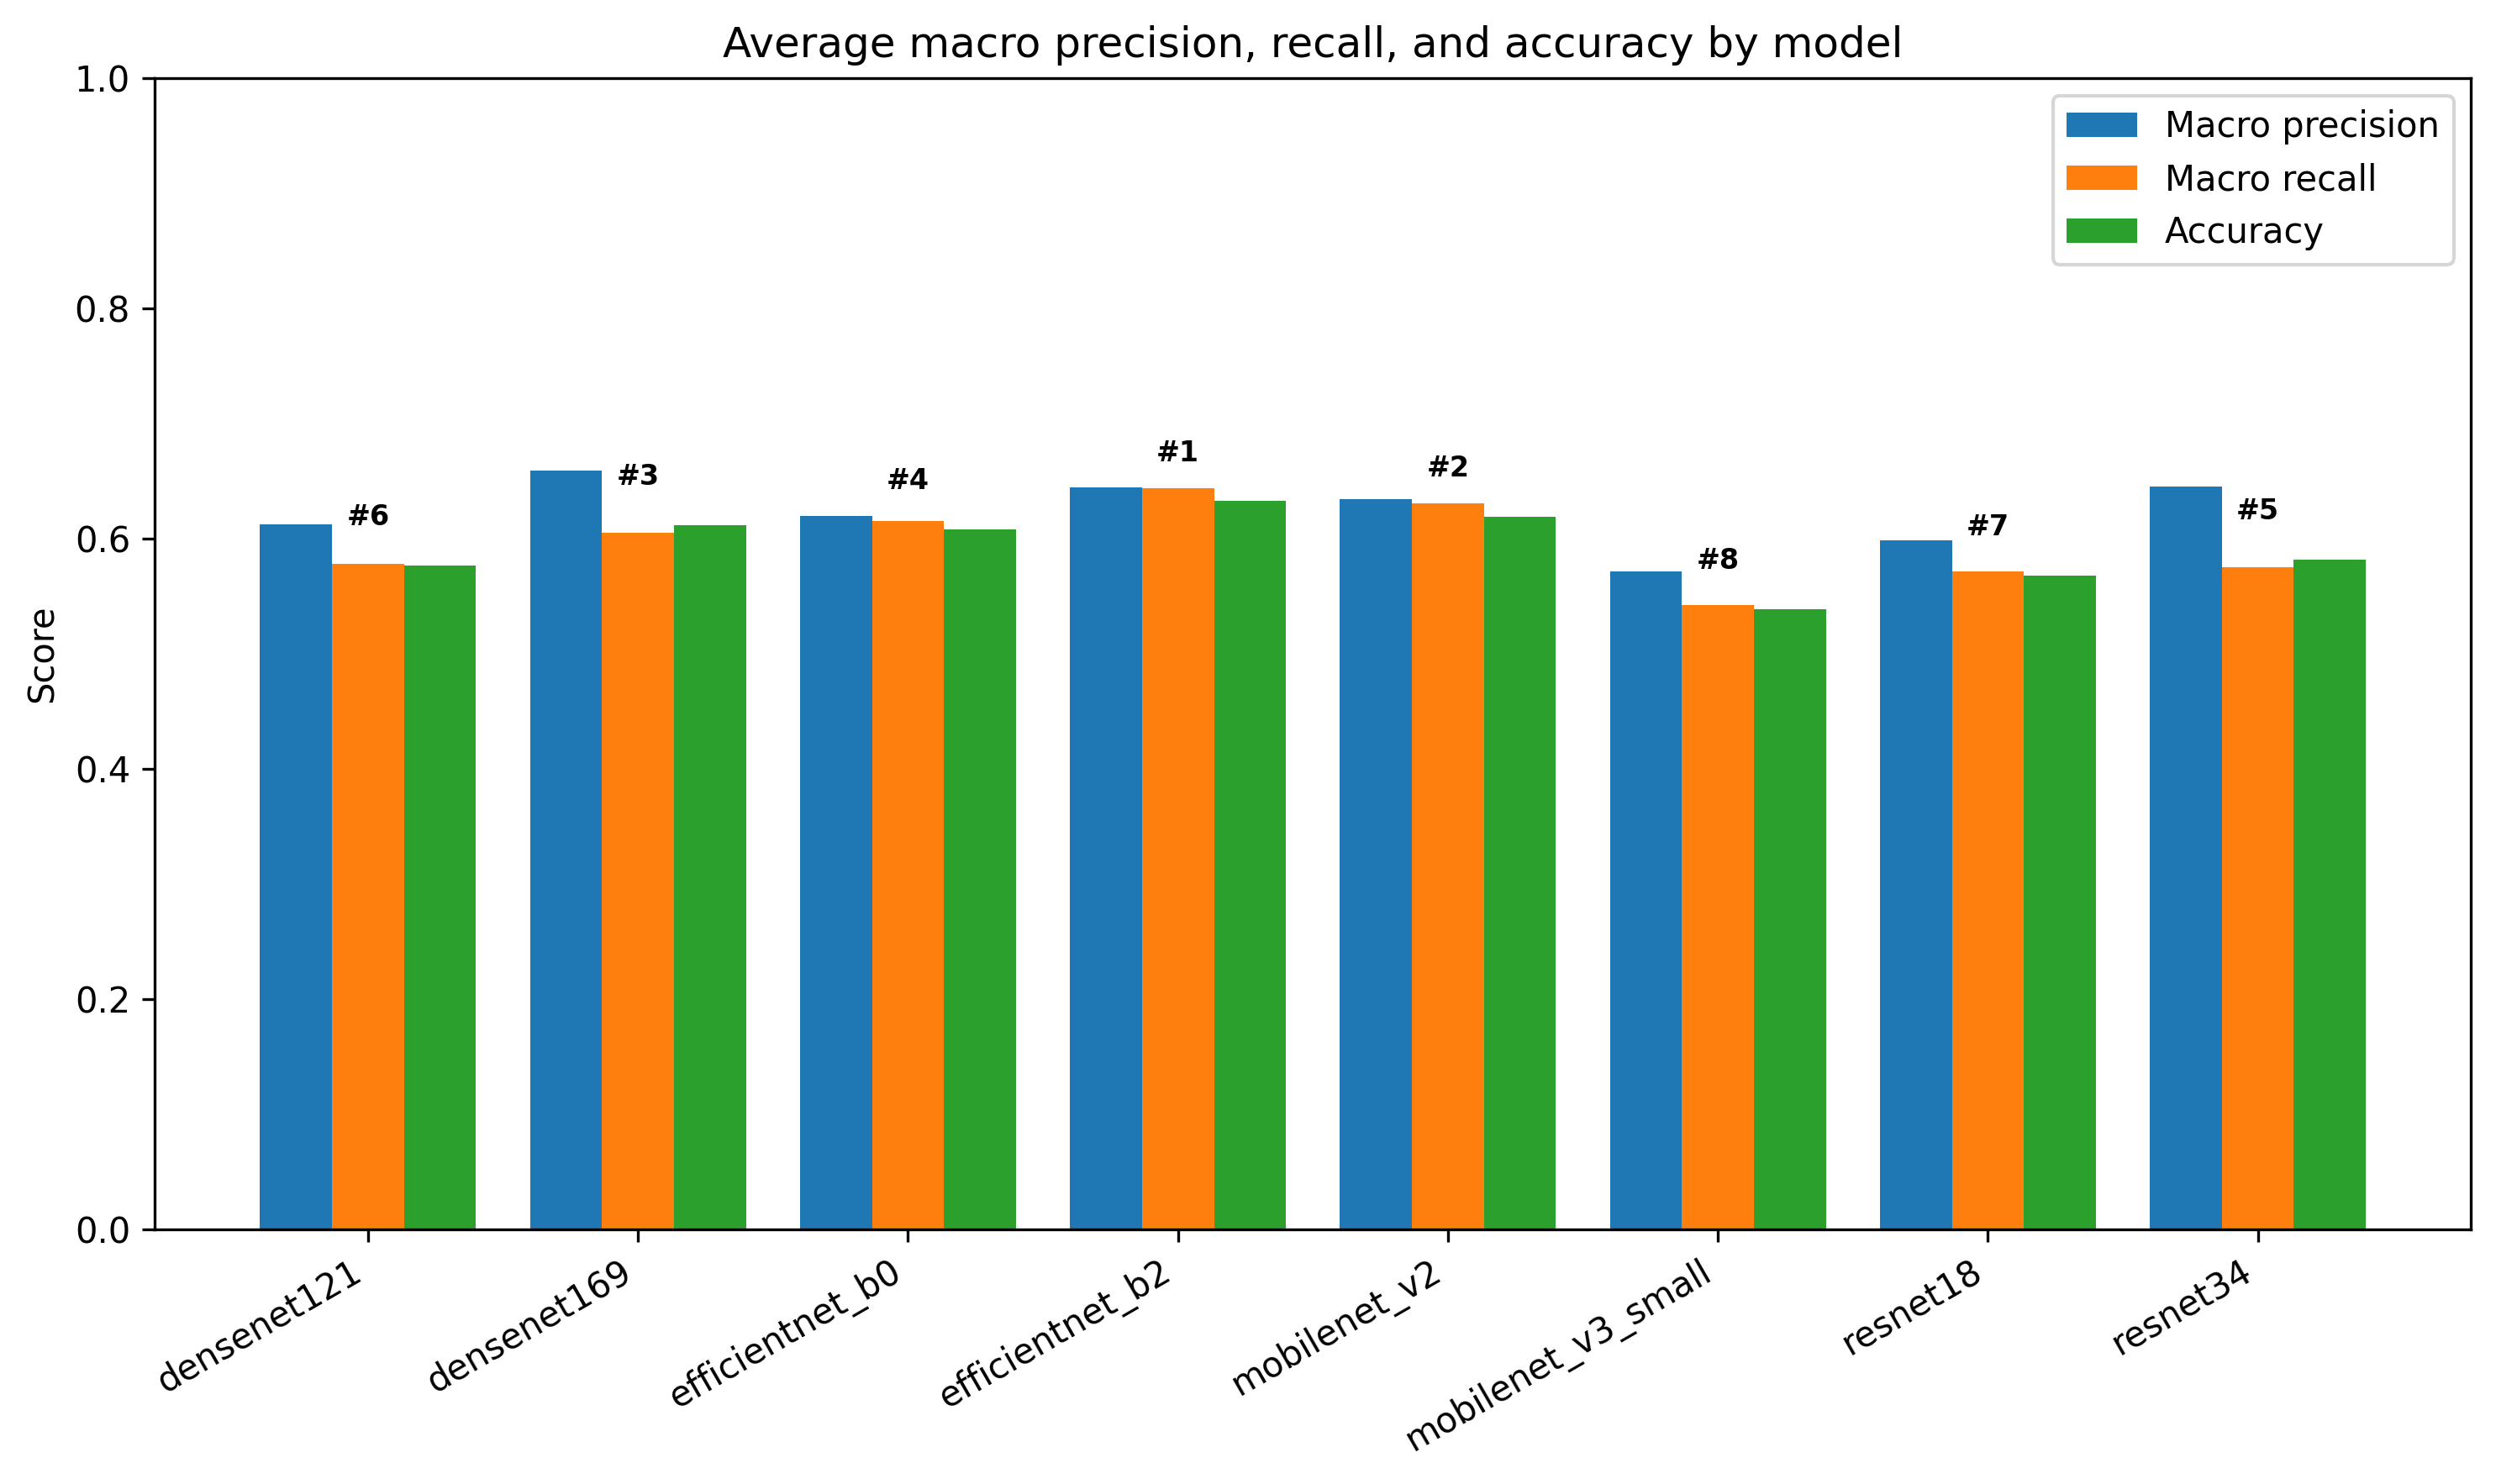
\includegraphics[width=\linewidth]{macro_metrics_by_model.png}
    \caption{Comparison of model families and sizes based on test accuracy, macro precision, and macro recall. Each bar represents the average performance across all training configurations for that model architecture.}
    \label{fig:model_family_size_comparison}
\end{figure}

What is important to note is that the overall performance of the different model architectures appears to be closely related to their ability to correctly classify the Blue class, which is the weakest class overall. This suggests that the ability to learn robust features for the Blue class may be an important factor in determining the overall performance of the models, and that architectures that are better able to capture and generalize from the visual features of the Blue class may tend to perform better overall. For example, EfficientNet B2, which shows the strongest overall performance, also has the highest accuracy for the Blue class, while MobileNet v3 small, which shows the weakest overall performance, also has the lowest accuracy for the Blue class. This suggests that improving performance on the Blue class may be an important area for future work in order to further improve the overall performance of the models on this dataset.

Furthermore, it is interesting to see that the larger models tend to outperform the smaller models on average, which suggests that larger models may not suffer from overfitting as much as one might expect in this small-data setting, and that they may be able to learn more robust features from the limited data available. However, there is still a lot of variability across training configurations for each architecture, and some smaller models perform better than some larger models on certain configurations. This suggests that while larger models may have an advantage in terms of capacity, they may also require more careful tuning of other design choices such as augmentation strength and freezing schedule in order to reach their full potential in the small-data regime.

\subsection{Overall Training Configuration Comparisons}

When comparing training configurations, we will analyze how each of the design choices (learning rate, augmentation strength, freezing schedule) impacts performance and whether there are any interactions between these choices and the model architecture. For example, it is possible that stronger augmentation may be more beneficial for smaller models than larger models, or that longer freezing schedules may be more effective for certain architectures than others. By analyzing these interactions, we can gain insights into which design choices are most important for improving generalization to unseen data in the small-data regime.

\begin{figure}
    \centering
    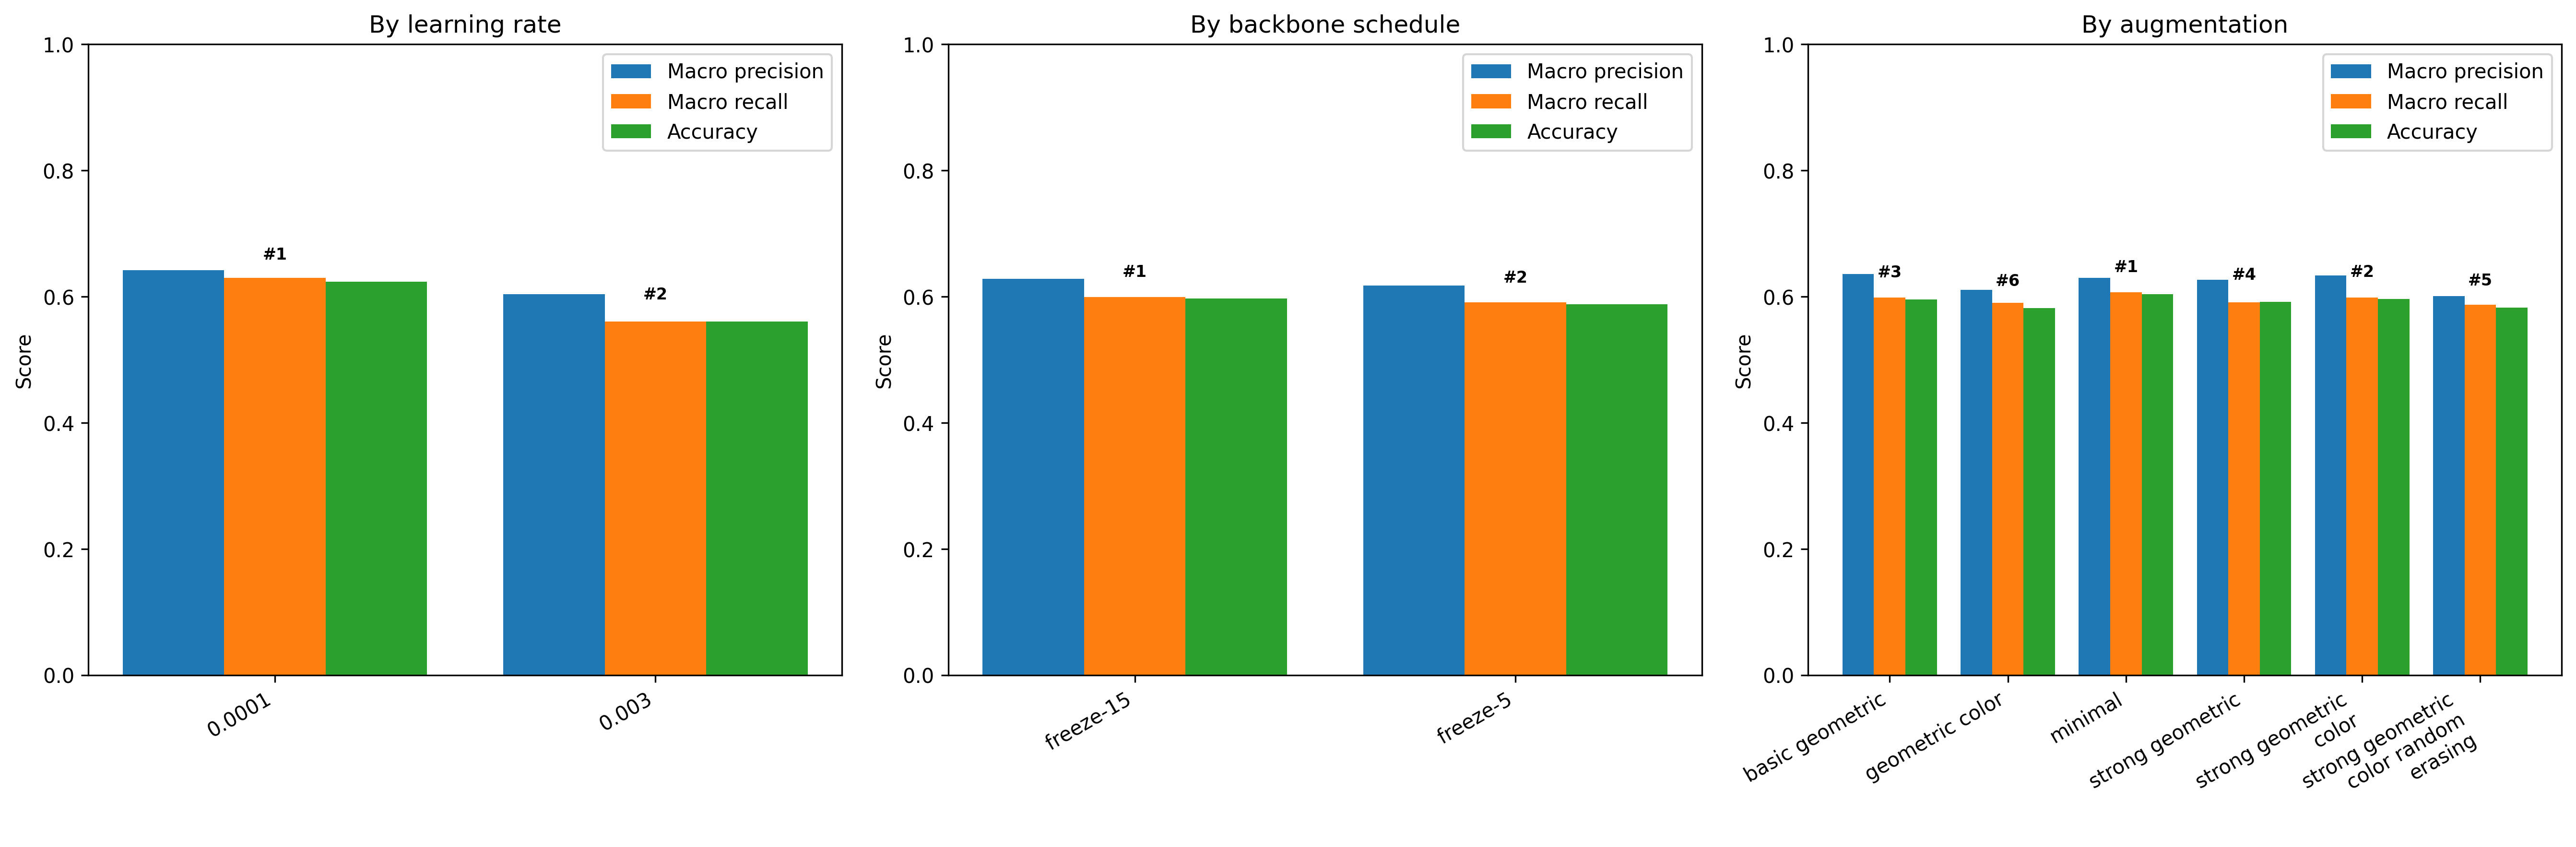
\includegraphics[width=\linewidth]{macro_metrics_by_strategy.png}
    \caption{Comparison of each training strategy (learning rate, augmentation strength, freezing schedule) based on test accuracy, macro precision, and macro recall. Each bar represents the average performance across all model architectures for that training strategy, with each of the other strategies varied.}
    \label{fig:training_config_comparison}
\end{figure}

See figure \ref{fig:training_config_comparison} for a summary of test accuracy, macro precision, and macro recall averaged across all model architectures for each training strategy. Surprisingly, augmentation strength does not show a clear trend in terms of improving performance, and in this sweep the strongest augmentation pipeline on average is a lack of augmentation. This suggests that stronger augmentation may not always be beneficial for improving generalization to unseen data in the small-data regime, and that it may be important to carefully consider the specific characteristics of the dataset and the task when designing augmentation strategies. Similarly, although the longer freezing schedule shows a marginal increase in performance, it is not large enough to suggest that it would always be beneficial. However, the learning rate does show a subtle trend, with the lower learning rate of $10^{-4}$ outperforming the higher learning rate of $3 \times 10^{-3}$. This suggests that using a lower learning rate may be an important design choice for improving generalization to unseen data in the small-data regime, as it may help prevent overfitting and allow the model to learn more robust features from the limited data available. This may especially be the case when fine-tuning pre-trained models, as a lower learning rate can help preserve the useful features learned from the larger source dataset while still allowing the model to adapt to the specific characteristics of the target dataset.

It is likely that the raw averages shown in figure \ref{fig:training_config_comparison} obscure important interactions between the training strategies and the model architectures. For example, it is possible that stronger augmentation may be more beneficial for smaller models than larger models, or that longer freezing schedules may be more effective for certain architectures than others. In fact, it may even be the case that stronger augmentation and longer freezing schedules can significantly improve performance for certain architectures while having little to no effect on other architectures, which could explain why there is no clear trend in the overall averages. Therefore, it will be important to analyze these interactions in more detail in order to gain a deeper understanding of how each training strategy impacts performance and how they interact with different model architectures in the small-data regime.

\subsection{Interactions Between Up To Two Design Choices}

When analyzing interactions between design choices, we will look at how pairs of design choices (e.g., backbone freezing schedule and augmentation strength) interact with each other and with model architecture to impact performance. For example, it is possible that stronger augmentation may be more beneficial for smaller models than larger models, or that longer freezing schedules may be more effective for certain architectures than others. By analyzing these interactions, we can gain insights into which combinations of design choices are most effective for improving generalization to unseen data in the small-data regime. We do not involve learning rates in this analysis because the overall trend for learning rates is clearer than for the other design choices. Furthermore, analyzing interactions between three or more design choices would be difficult to interpret and may even be a result of random noise rather than meaningful patterns, so we will limit our analysis to interactions between pairs of design choices.

\subsubsection{Interaction Between Backbone Freezing Schedule and Augmentation Strength}

First, we will analyze the interaction between backbone freezing schedule and augmentation strength. See figure \ref{fig:freeze_aug_interaction} for a summary of test accuracy, macro precision, and macro recall averaged across all model architectures for each combination of freezing schedule and augmentation strength. There does not appear to be a clear trend in terms of which combinations of freezing schedule and augmentation strength are most effective for improving performance, which suggests that there may not be a strong interaction between these two design choices in terms of their impact on performance. To summarize, the combination of freezing for the first 15 epochs and the strong geometric + color augmentation pipeline shows the highest average performance, while the combination of freezing for the first 15 epochs and the strong geometric + color + random erasing augmentation pipeline shows the lowest average performance. However, the differences in performance between these combinations are relatively small, and there is a lot of variability across model architectures for each combination.

\begin{figure}
    \centering
    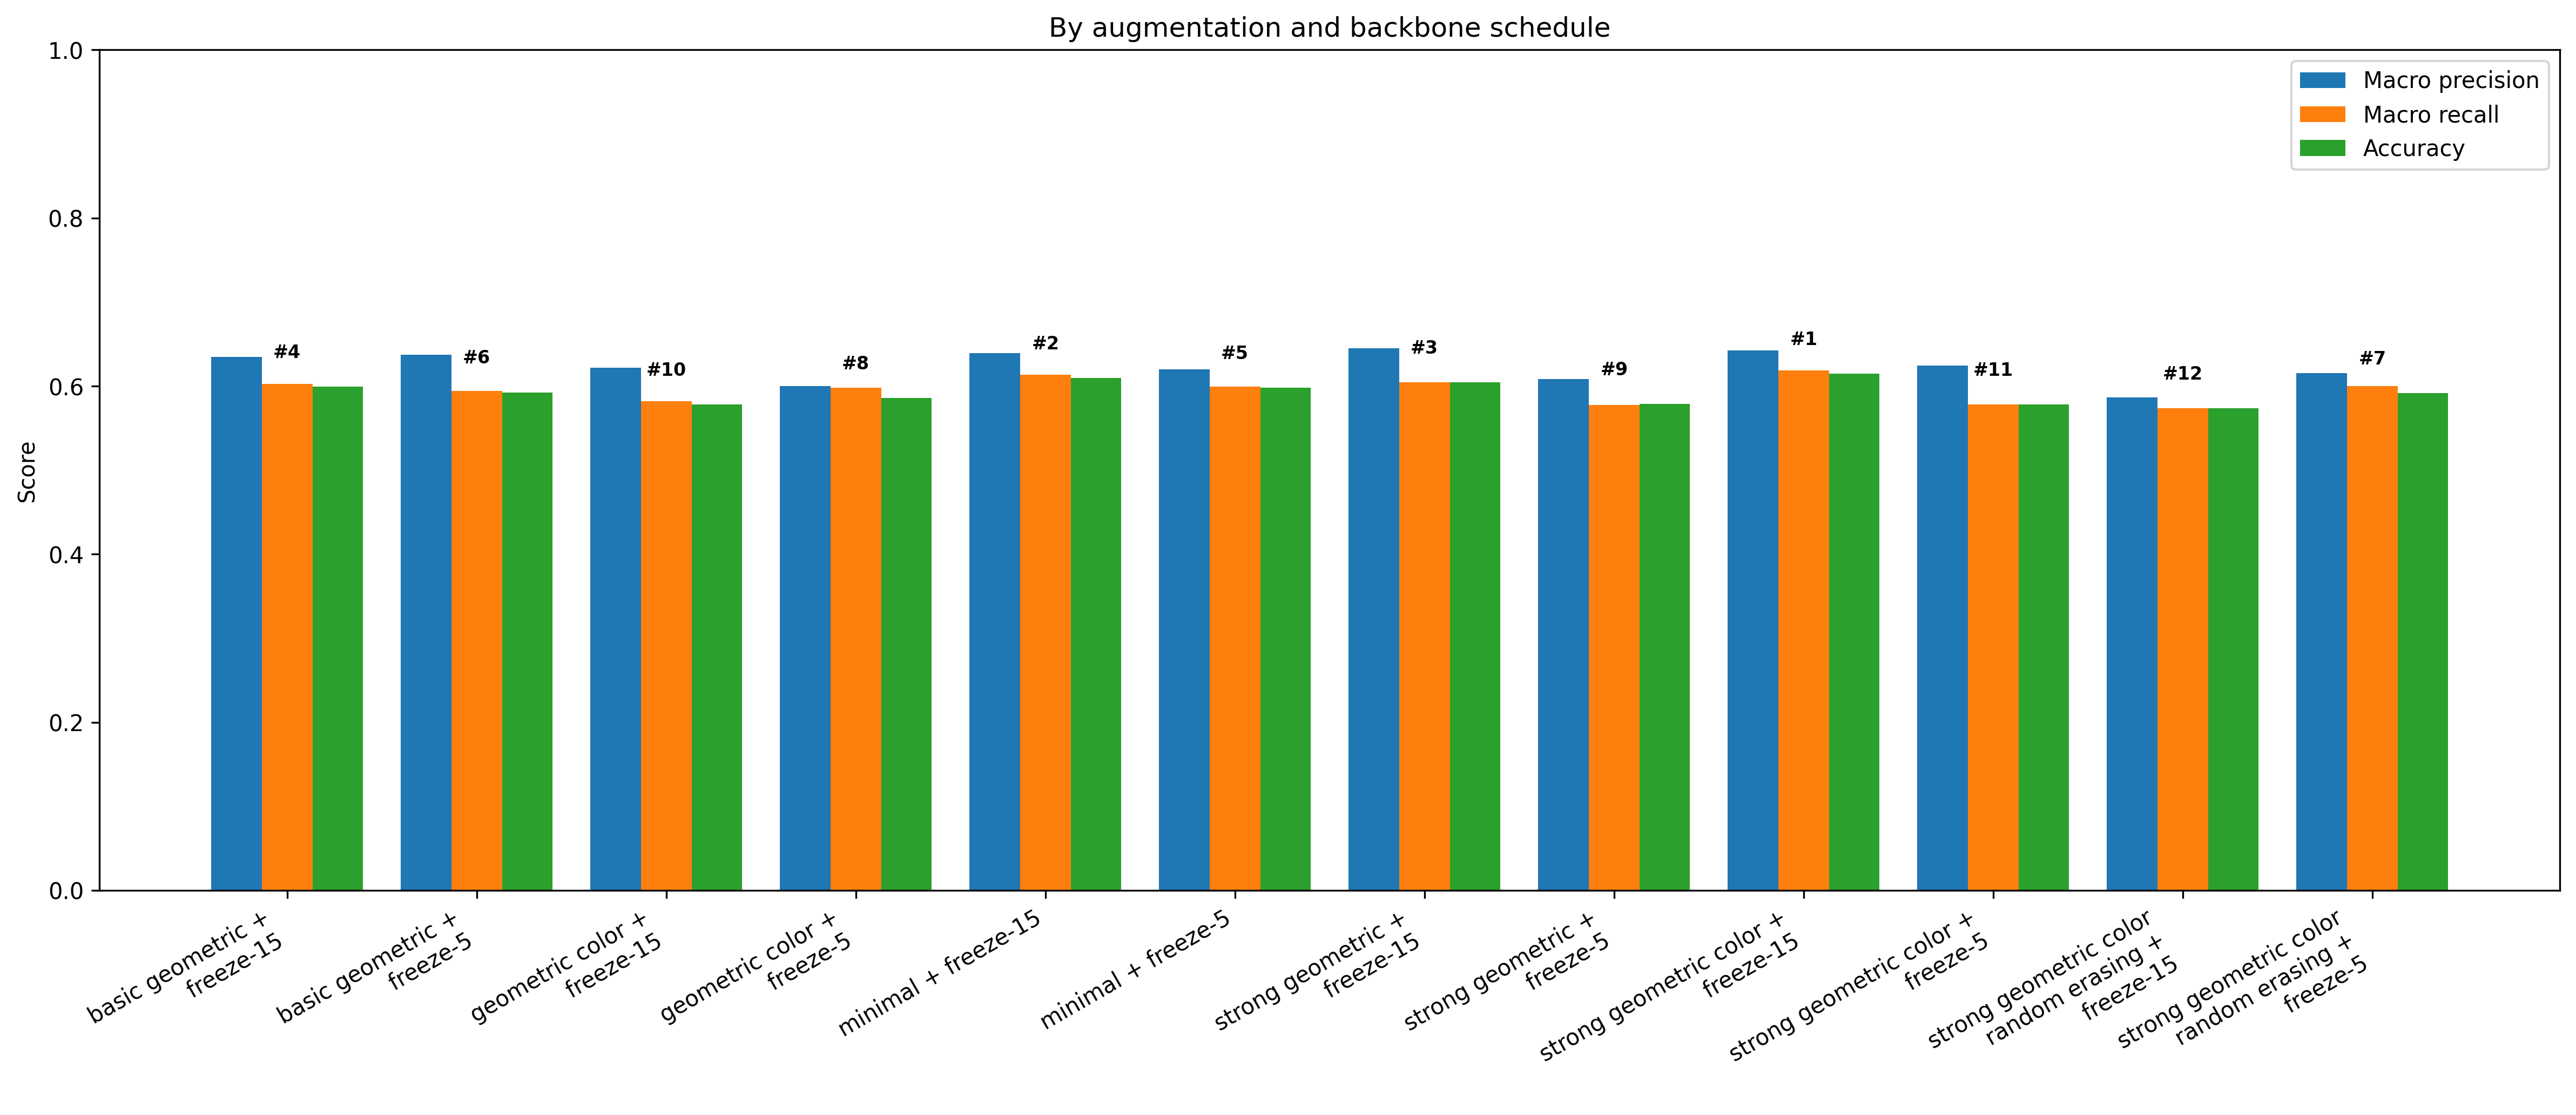
\includegraphics[width=\linewidth]{macro_metrics_by_augmentation_freeze_combo.png}
    \caption{Interaction between backbone freezing schedule and augmentation strength based on test accuracy, macro precision, and macro recall. Each set of bars represents the average performance across all model architectures for that combination of freezing schedule and augmentation strength, with the learning rate varied.}
    \label{fig:freeze_aug_interaction}
\end{figure}

\subsubsection{Interaction Between Backbone Freezing Schedule and Model Architecture}

It may also be useful to analyze the interaction between backbone freezing schedule and model architecture. See figure \ref{fig:freeze_arch_interaction} for a summary of test accuracy, macro precision, and macro recall averaged across all training configurations for each combination of freezing schedule and model architecture. There does not appear to be a clear trend in terms of which combinations of freezing schedule and model architecture are most effective for improving performance, which suggests that there may not be a strong interaction between these two design choices in terms of their impact on performance. In fact, the two strongest combinations are both EfficientNet B2, which is the strongest architecture overall, with one of the freezing schedules each. The two weakest combinations are both MobileNet v3 small, which is the weakest architecture overall, with one of the freezing schedules each. In general, most models show similar performance across both freezing schedules, which suggests that the choice of freezing schedule may not have a strong impact on performance for most architectures in the small-data regime.

Despite this, 7 out of 8 models show marginally stronger performance with the longer freezing schedule than with the shorter freezing schedule, which suggests that longer freezing schedules may be somewhat more beneficial for improving performance across a range of architectures in the small-data regime, even if the overall trend is not strong enough to be clearly visible in the averages shown in figure \ref{fig:training_config_comparison}. This may be because longer freezing schedules allow the model to better preserve the useful features learned from the larger source dataset while still allowing for some adaptation to the specific characteristics of the target dataset, which can help improve generalization to unseen data in the small-data regime.

\begin{figure}
    \centering
    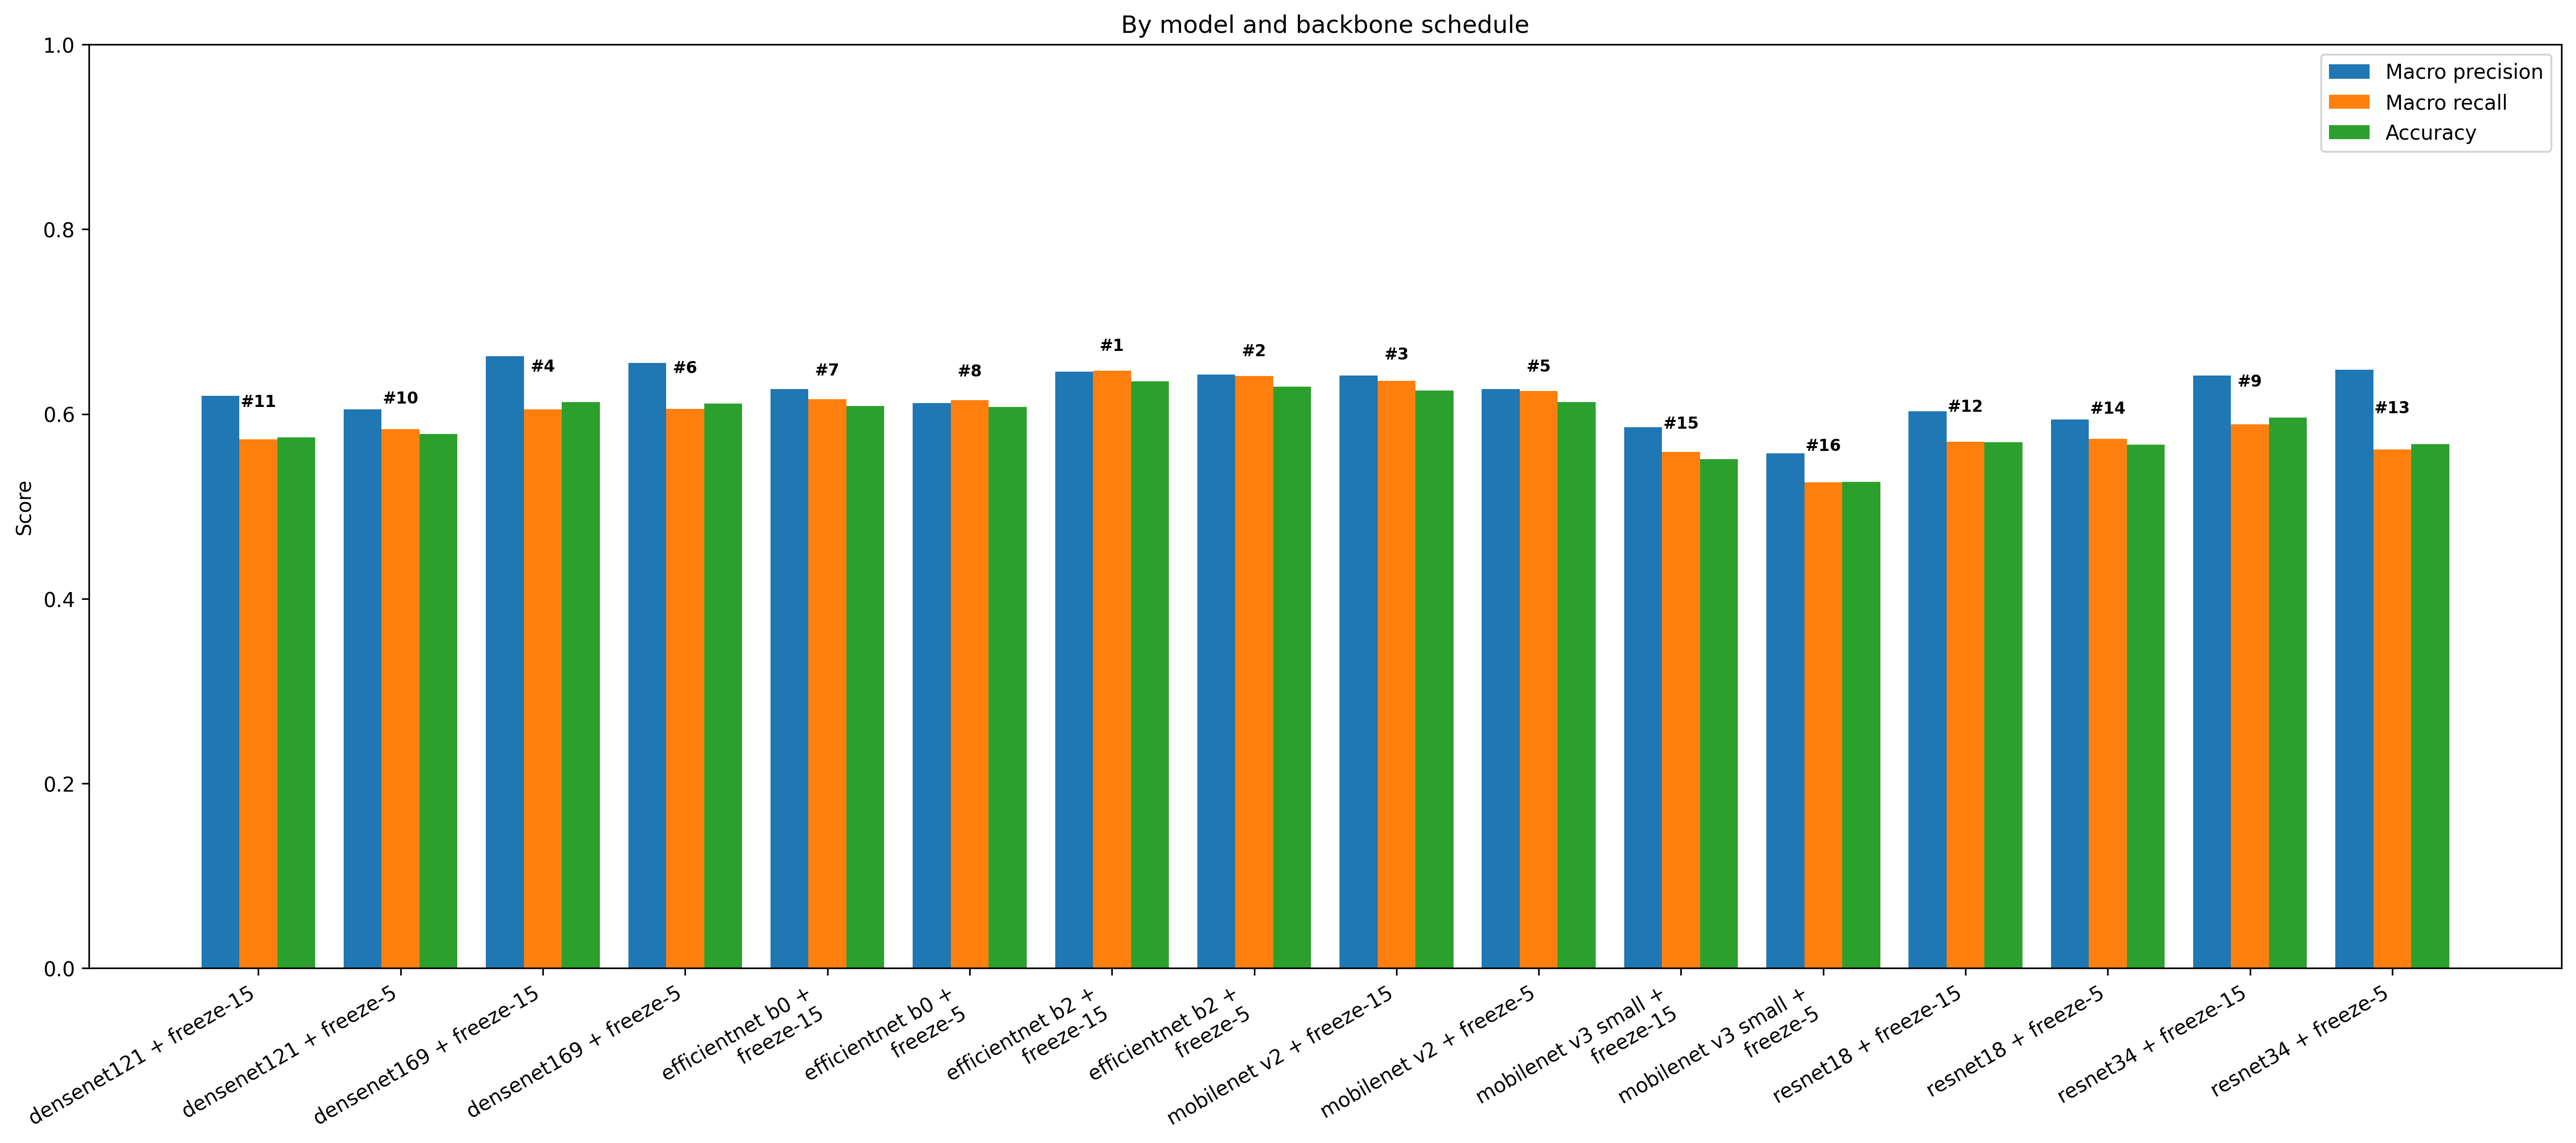
\includegraphics[width=\linewidth]{macro_metrics_by_model_freeze_combo.png}
    \caption{Interaction between backbone freezing schedule and model architecture based on test accuracy, macro precision, and macro recall. Each set of bars represents the average performance across all training configurations for that combination of freezing schedule and model architecture, with the learning rate and augmentation strength varied.}
    \label{fig:freeze_arch_interaction}
\end{figure}

\subsubsection{Interaction Between Augmentation Strength and Model Architecture}

Finally, it may be useful to analyze the interaction between augmentation strength and model architecture. See figure \ref{fig:aug_arch_interaction} for a summary of test accuracy, macro precision, and macro recall averaged across all training configurations for each combination of augmentation strength and model architecture. Note that the three weakest augmentation strategies are pooled together, as well as the three strongest augmentation strategies. There does not appear to be a clear trend in terms of which combinations of augmentation strength and model architecture are most effective for improving performance, which suggests that there may not be a strong interaction between these two design choices in terms of their impact on performance. In general, most models show similar performance across different augmentation strengths, which suggests that the choice of augmentation strength may not have a strong impact on performance for most architectures in the small-data regime.



\begin{figure}
    \centering
    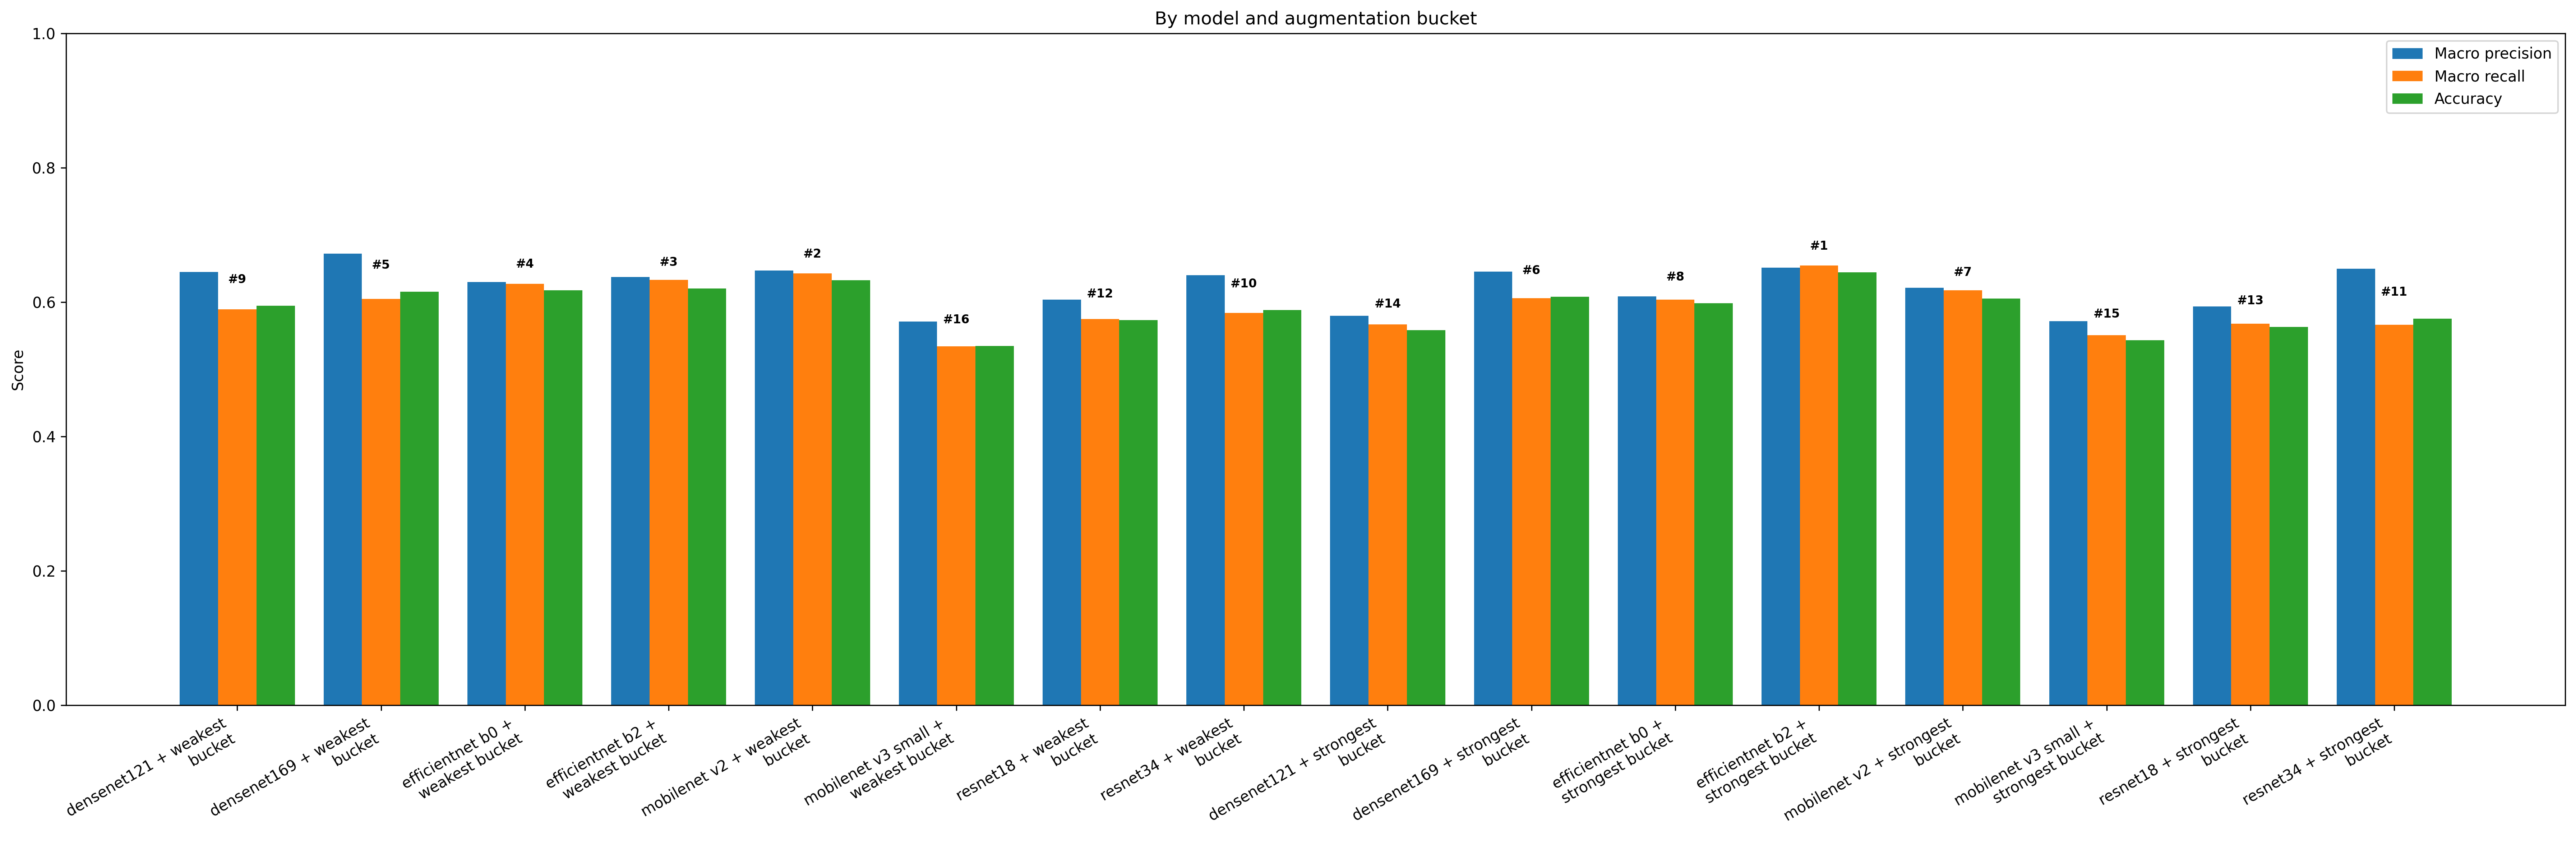
\includegraphics[width=\linewidth]{macro_metrics_by_model_augmentation_extremes.png}
    \caption{Interaction between augmentation strength and model architecture based on test accuracy, macro precision, and macro recall. Each set of bars represents the average performance across all training configurations for that combination of augmentation strength and model architecture, with the learning rate and freezing schedule varied. The three weakest augmentation strategies (minimal, basic geometric, and strong geometric) are pooled together, as well as the three strongest augmentation strategies (basic geometric + color, strong geometric + color, and strong geometric + color + random erasing).}
    \label{fig:aug_arch_interaction}
\end{figure}

\section{Discussion}
The discussion will focus on which design choices appear most beneficial in the small-data regime and which choices seem to encourage overfitting or unstable generalization. Particular attention will be paid to whether stronger augmentation improves robustness across individuals, whether lighter-weight architectures outperform larger ones on this dataset, and how much performance varies across classes with different levels of representation.

\subsection{Benefits of Design Choices}

Overall, the results suggest that using a lower learning rate may allow for more stable generalization to unseen data in the small-data regime, as it may help prevent overfitting and allow the model to learn more robust features from the limited data available. This may especially be the case when fine-tuning pre-trained models, as a lower learning rate can help preserve the useful features learned from the larger source dataset while still allowing the model to adapt to the specific characteristics of the target dataset.

However, the results do not show a clear trend in terms of which augmentation strategies are most effective for improving performance, which suggests that stronger augmentation may not always be beneficial for improving generalization to unseen data in the small-data regime. In fact, they suggest that an increase in augmentation strength can sometimes harm performance on this dataset. This may be a characteristic of this specific dataset and task, and it may be important to carefully consider the specific characteristics of the dataset and the task when designing augmentation strategies. Similarly, although the longer freezing schedule shows a marginal increase in performance, it is not large enough to suggest that it would always be beneficial. However, it may still be worth considering longer freezing schedules as a potential strategy for improving performance in the small-data regime, as they may allow the model to better preserve the useful features learned from the larger source dataset while still allowing for some adaptation to the specific characteristics of the target dataset.

It is important to consider the limitations of this study when interpreting the results. Further work may include expanding the dataset, incorporating more formal genetic labels, or even using an entirely different dataset to see if the trends observed here hold in other contexts. Additionally, it may be worth exploring other design choices such as cross-validation, class-balanced losses, or self-supervised pretraining to see if they can further improve performance in the small-data regime.

\subsection{Choice of Model Architecture}

The results suggest that the choice of model architecture can have a significant impact on performance in the small-data regime, with larger models within the same family generally performing better. In fact, they suggest that the choice of model architecture may be more important than the choice of training strategy in this sweep, as the differences in performance between different model architectures are much larger than the differences in performance between different training strategies. However, there is still a lot of variability across training configurations for each architecture, and some models that perform worse on average can outperform some models that perform better on average on certain configurations (see figures \ref{fig:freeze_aug_interaction}, \ref{fig:aug_arch_interaction}, \ref{fig:freeze_arch_interaction}). This suggests that while larger models may have an advantage in terms of capacity, they may also require more careful tuning of other design choices such as augmentation strength and freezing schedule in order to achieve their full potential in the small-data regime.

\begin{figure}
    \centering
    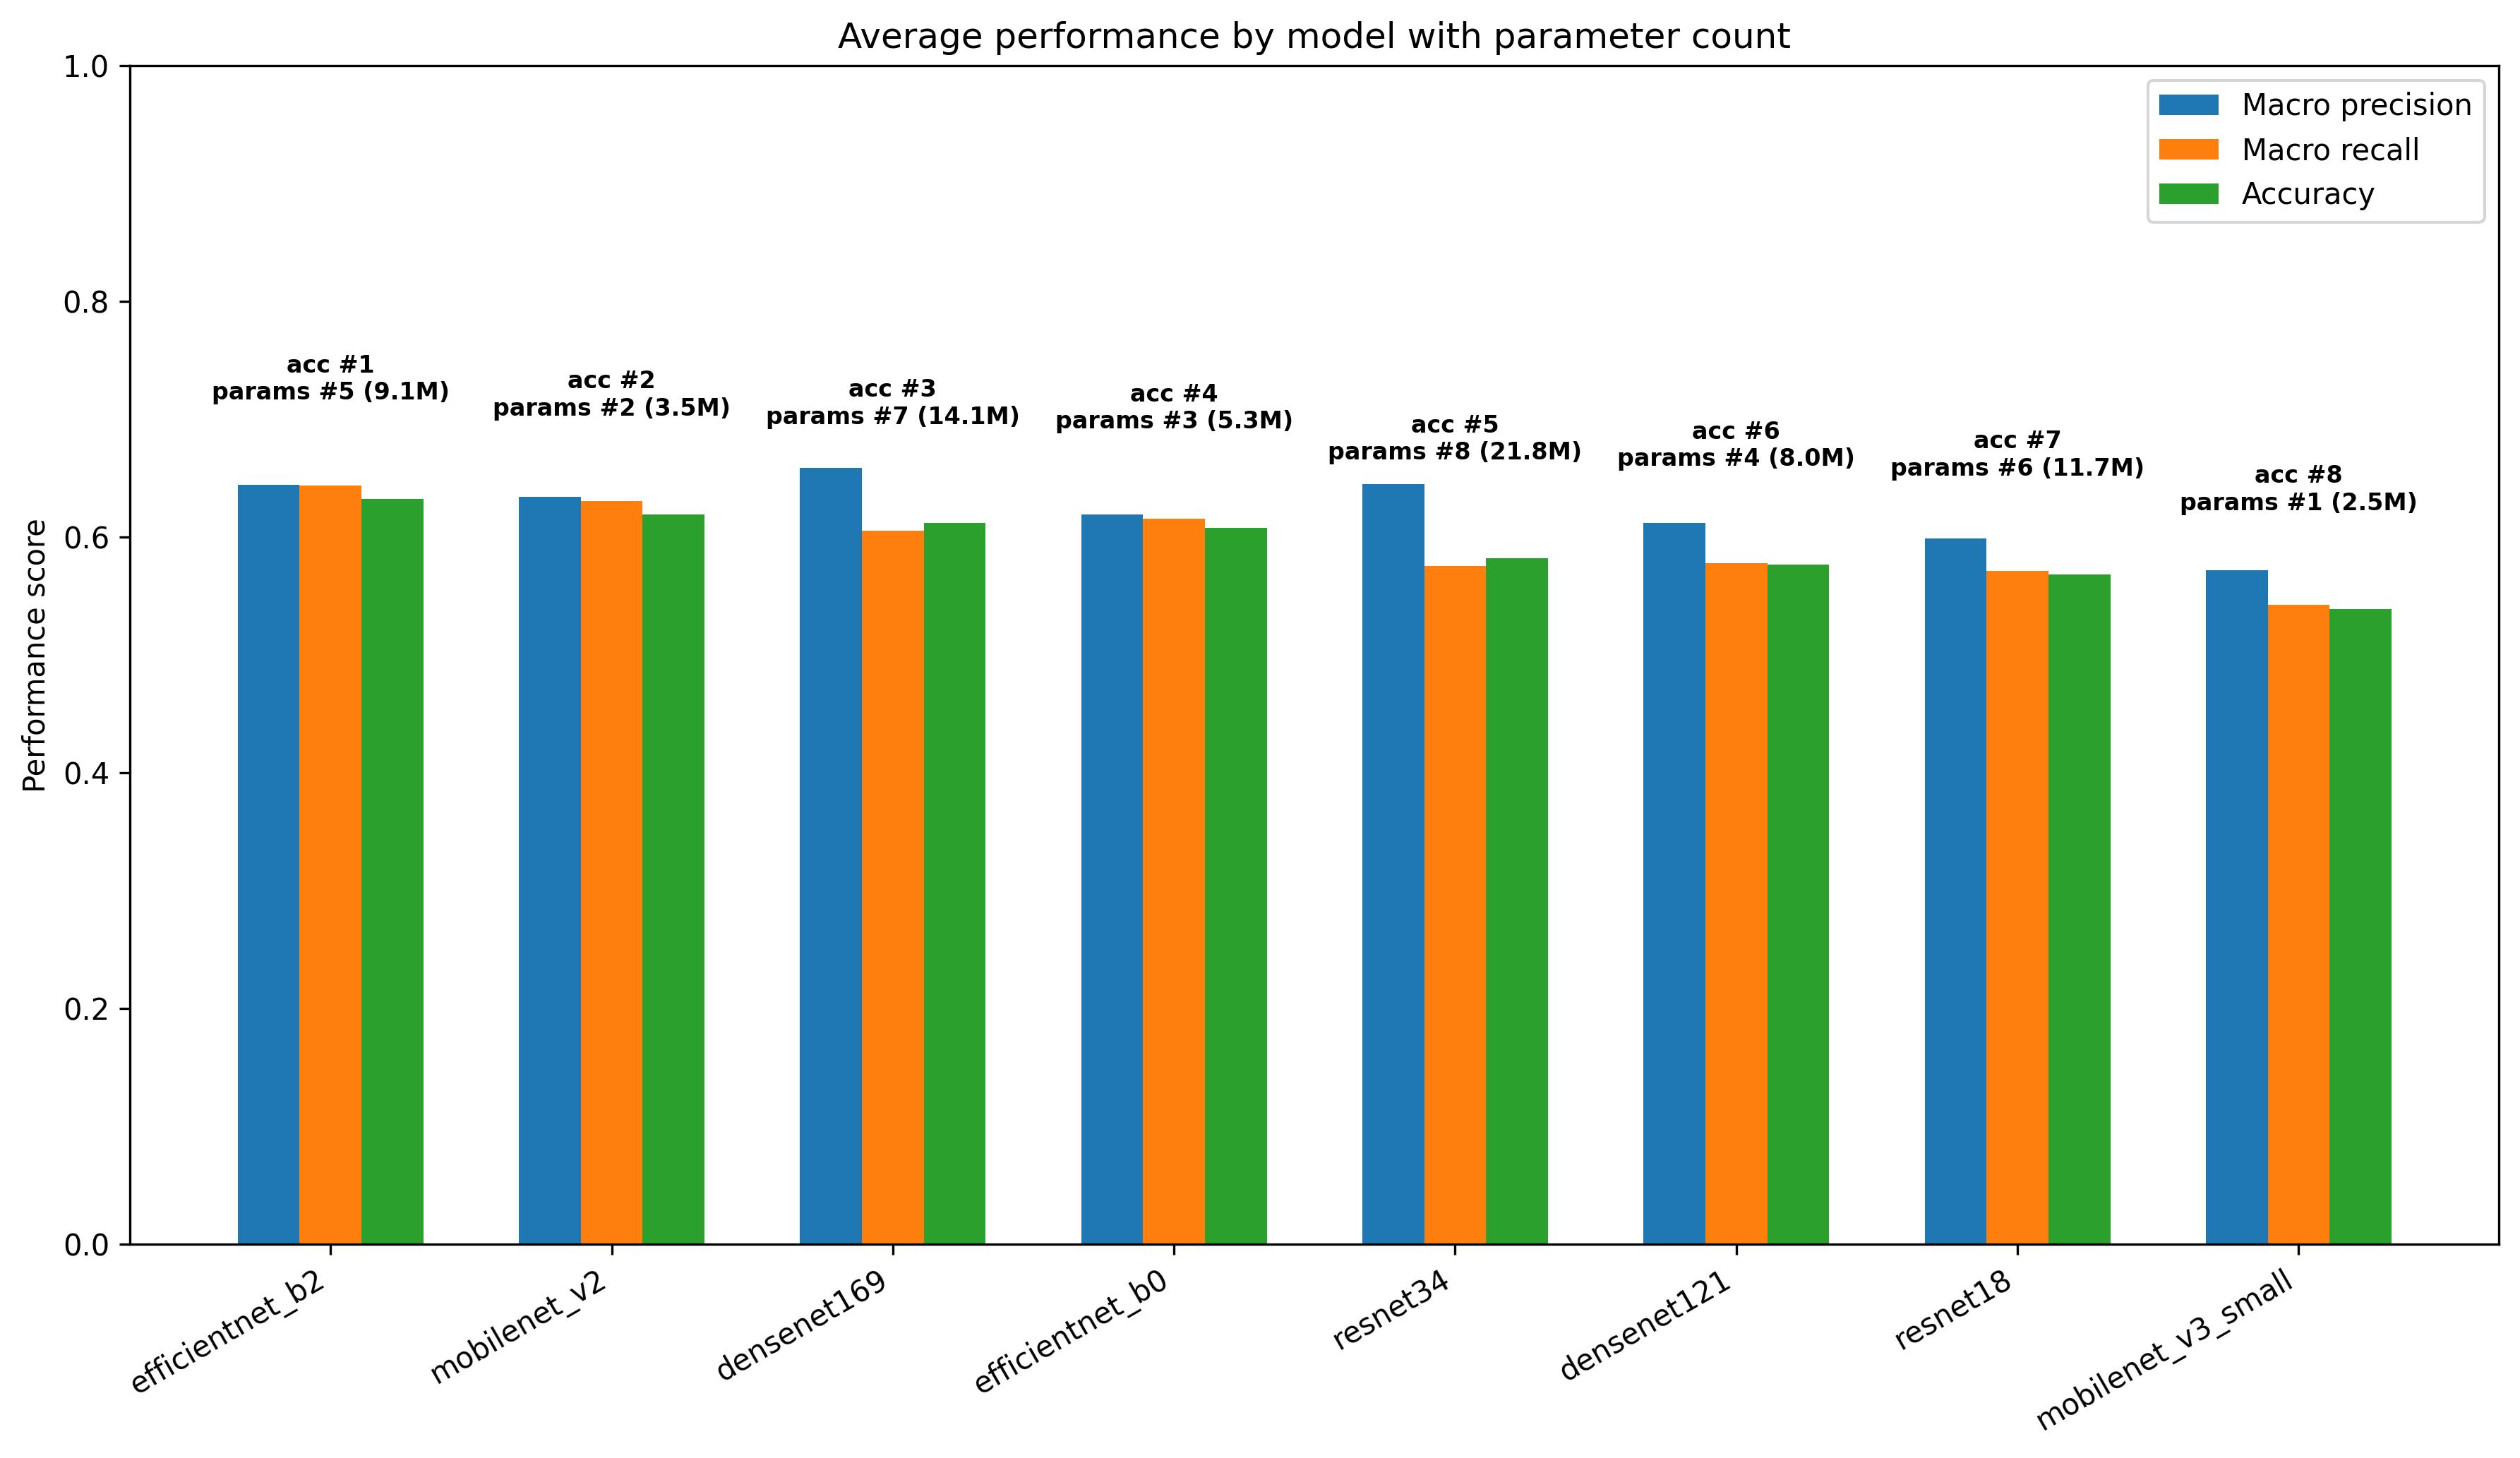
\includegraphics[width=\linewidth]{macro_metrics_by_model_with_params.png}
    \caption{Comparison of model families and sizes based on test accuracy, macro precision, and macro recall. Each bar represents the average performance across all training configurations for that model architecture. The larger models within each family tend to perform better than the smaller models within the same family, which suggests that larger models may be able to learn more robust features from the limited data available in the small-data regime. Figure also shows the parameter count for each model architecture, which is a common measure of model size.}
    \label{fig:model_family_size_params_comparison}
\end{figure}

Although larger models within the same family perform better than their smaller counterparts, larger models by raw parameter count do not necessarily perform better than smaller models from a different family. For example, ResNet-34 is the model with the largest parameter count, but it places fifth overall in terms of performance, while MobileNet v2 is the model with the second smallest parameter count, but it places second overall in terms of performance (see figure \ref{fig:model_family_size_params_comparison}). This suggests that the choice of model family may be more important than the choice of model size within a family, and that certain architectures may be better suited for learning robust features from limited data than others. For example, EfficientNet B2 shows the strongest overall performance, which may be due to its efficient architecture and ability to learn robust features from limited data, while MobileNet v3 small shows the weakest overall performance, which may be due to its smaller capacity and less effective architecture for learning from limited data.

\subsection{Limitations and Future Work}

As mentioned, there are several limitations to this study that should be considered when interpreting the results. The first and most obvious limitation is the dataset itself. Although it is intentionally designed to be small with class imbalance, it is clear from Section \ref{sec:per_class_performance} that models perform much better on some classes than others, and that the overall performance of the models appears to be closely tied to their ability to learn robust features for just one of the classes (the Blue class). This suggests that the dataset may not be sufficiently representative of the broader problem of small-data image classification, and that the trends observed here may not generalize to other datasets or tasks. Future work could involve expanding the dataset to include more classes, more individuals per class, and more images per individual in order to create a more balanced and representative dataset for studying small-data image classification.

Furthermore, it is possible that we have unfairly dismissed the possible benefits of stronger augmentation due to the specific characteristics of this dataset and task. For example, it may be the case that stronger augmentation does consistently improve performance at true generalization to data outside of our dataset, but that it does not improve performance on our test set because the test set is not sufficiently representative of the broader distribution of data that we are trying to generalize to. Future work could involve testing the models on a more diverse and representative test set in order to better understand the potential benefits of stronger augmentation for improving generalization to unseen data in the small-data regime.

Finally, there are many other design choices that we did not explore in this study that could potentially have a significant impact on performance in the small-data regime. For example, it may be worth exploring other training strategies such as cross-validation, class-balanced losses, or self-supervised pretraining to see if they can further improve performance in the small-data regime. Additionally, it may be worth exploring other model architectures beyond the four families that we evaluated in this study to see if there are other architectures that are better suited for learning robust features from limited data. Overall, while this study provides some insights into the impact of certain design choices on performance in the small-data regime, there is still much work to be done in order to fully understand how to best approach small-data image classification and to identify the most effective strategies for improving generalization to unseen data in this challenging setting.

\section{Conclusion}

In this work, we have conducted a surface-level exploration of the impact of different design choices of object classification models in the small-data regime. We evaluated four different model families with two size variants each, and we explored the impact of three different training strategies (learning rate, augmentation strength, freezing schedule) on performance. Our results suggest that the choice of model architecture can have a significant impact on performance in the small-data regime, with larger models within the same family generally performing better. However, there is still a fair amount of variability across training configurations for each architecture, and some models that perform worse on average can outperform some models that perform better on average on certain configurations. We also found that using a lower learning rate may be an important design choice for improving generalization to unseen data in the small-data regime, while stronger augmentation and longer freezing schedules do not show clear trends in terms of their impact on performance. Finally, we found that performance varies significantly across classes within the dataset, with some classes being much easier for the models to learn robust features for than others. Our recommendation for practitioners working in the small-data regime is to carefully consider the choice of model architecture and to experiment with different training strategies, but that in this sweep the choice of model architecture appears to have a much larger impact on performance than the choice of training strategy, and that it may be worth investing more time in selecting and tuning the model architecture than in fine-tuning training strategies.

\section*{Acknowledgment}
We gratefully acknowledge the breeders who gave permission for their rat images to be included in this dataset. These breeders include:

\begin{itemize}
    \item Kolohe 'Iole Rattery - \href{https://koloheiolerattery.com/}{koloheiolerattery.com}
    \item Little Paws Rattery - \href{https://iowalittlepawsrattery.weebly.com/}{littlepawsrattery.weebly.com}
\end{itemize}

We ask that you please consider supporting these breeders if you find this work useful, as they are the ones who made this dataset possible by sharing their photographs of their rats. The code used to run the experiments in this paper is available at \url{https://github.com/NathanWithNoCathan/RatClass}. The repository includes the code for the dataset splitting procedure, the training and evaluation pipelines, the code for generating the figures, and the dataset.

\bibliographystyle{IEEEtran}
\bibliography{references}

\end{document}